%% ****** Start of file apstemplate.tex ****** %
%%
%%
%%   This file is part of the APS files in the REVTeX 4.2 distribution.
%%   Version 4.2a of REVTeX, January, 2015
%%
%%
%%   Copyright (c) 2015 The American Physical Society.
%%
%%   See the REVTeX 4 README file for restrictions and more information.
%%
%
% This is a template for producing manuscripts for use with REVTEX 4.2
% Copy this file to another name and then work on that file.
% That way, you always have this original template file to use.
%
% Group addresses by affiliation; use superscriptaddress for long
% author lists, or if there are many overlapping affiliations.
% For Phys. Rev. appearance, change preprint to twocolumn.
% Choose pra, prb, prc, prd, pre, prl, prstab, prstper, or rmp for journal
%  Add 'draft' option to mark overfull boxes with black boxes
%  Add 'showkeys' option to make keywords appear
%\documentclass[aps,prfluids,preprint,superscriptaddress]{revtex4-2}
%\documentclass[aps,prl,preprint,superscriptaddress]{revtex4-2}
\documentclass[aps,prfluids,reprint,superscriptaddress]{revtex4-2}

\usepackage{graphicx}
\usepackage[hypertexnames=false,
pdfstartview=FitH,
breaklinks=true,
bookmarks=true,
bookmarksopen=true,
bookmarksnumbered=true]{hyperref}
\urlstyle{same}
\hypersetup{
	colorlinks = true,
	linkcolor  = blue,
	urlcolor   = blue,
	citecolor  = blue,
}
\setlength{\parskip}{0cm plus4mm minus2mm}
\setlength{\bibsep}{-1.45pt}



\usepackage{natbib}

%user defined commands
\newcommand{\h}[1]{\textbf{\textit{#1}}}
\newcommand{\ii}[1]{\text{#1}}
\newcommand{\noi}{\noindent}
\newcommand{\nn}{\nonumber}
\newcommand{\overbar}[1]{\mkern 1.5mu\overline{\mkern-2mu#1\mkern-2mu}\mkern 1.5mu}
%for roman numeral
\newcommand{\RN}[1]{%
	\textup{\uppercase\expandafter{\romannumeral#1}}%
}
\newcommand{\Rn}[1]{%
	\textup{\expandafter{\romannumeral#1}}%
}
\renewcommand{\textrm}{\rm}
\usepackage{siunitx} % JCBdM: I add this to avoid incompatibility
\usepackage{bm} % Bold in math mode
\usepackage{amsmath} %extra math packages
\usepackage{amssymb} %for math symbols
\usepackage{physics} %for partial differential equations
\DeclareDocumentCommand\dpdv{}{\displaystyle\partialderivative}
\usepackage{multirow}
\usepackage{cancel}
\usepackage{scalerel} %change size of subscripts
\usepackage{soul,color}
%\usepackage{ulem}
\usepackage{xcolor}

\newcommand{\Wietze}[1]{\textcolor{teal}{#1}}
\newcommand{\red}[1]{\textcolor{red}{#1}}

\DeclareRobustCommand{\hly}[1]{{\sethlcolor{yellow}\hl{#1}}}
\DeclareRobustCommand{\hlr}[1]{{\sethlcolor{pink}\hl{#1}}}

%tikz
\usepackage{pgfplots, tikz}
\usetikzlibrary{3d}
\usepackage{tikz-3dplot}
\pgfplotsset{compat=newest} 
\usetikzlibrary{shapes.geometric}
\usetikzlibrary{arrows.meta}
\usetikzlibrary{positioning}
\usepgfplotslibrary{external}
%\tikzexternalize[prefix=cache/]

\pgfplotsset{colormap={bwr}{
		rgb(0)=(0.0, 0.0, 1.0),
		rgb(25)=(0.2, 0.2, 1.0),
		rgb(51)=(0.4, 0.4, 1.0),
		rgb(76)=(0.6, 0.6, 1.0),
		rgb(102)=(0.8, 0.8, 1.0),
		rgb(127)=(1.0, 1.0, 1.0),
		rgb(153)=(1.0, 0.8, 0.8),
		rgb(178)=(1.0, 0.6, 0.6),
		rgb(204)=(1.0, 0.4, 0.4),
		rgb(230)=(1.0, 0.2, 0.2),
		rgb(255)=(1.0, 0.0, 0.0),
}}
\definecolor{deepskyblue}{rgb}{0.000, 0.749, 1.000}
\definecolor{orange}{rgb}{1.000, 0.647, 0.000}
\definecolor{mediumseagreen}{rgb}{0.235, 0.702, 0.443}
\definecolor{slateblue}{rgb}{0.420, 0.353, 0.804}
\definecolor{crimson}{rgb}{0.863, 0.078, 0.235}
\definecolor{skyblue}{rgb}{0.529, 0.808, 0.922}
\definecolor{tomato}{rgb}{1.000, 0.388, 0.278}
\definecolor{blueviolet}{rgb}{0.54117647, 0.16862745, 0.88627451}

\definecolor{orangered}{rgb}{1.0, 0.2706, 0.0}
\definecolor{darkorange}{rgb}{1.0, 0.5490, 0.0}
\definecolor{dimgrey}{rgb}{0.4118, 0.4118, 0.4118}
\definecolor{k}{rgb}{0, 0, 0}

\usepackage{mdframed}
\usepackage{hhtensor}

\usepackage{cleveref}

\newcommand{\subref}[2]{\ref{#1}\hyperref[#1]{(#2)}}

\begin{document}

% Use the \preprint command to place your local institutional report
% number in the upper righthand corner of the title page in preprint mode.
% Multiple \preprint commands are allowed.
% Use the 'preprintnumbers' class option to override journal defaults
% to display numbers if necessary
%\preprint{}

%Title of paper
\title{Magnetic damping of standing waves in rectangular geometries}


\author{Pranav Hegde}
\affiliation{Helmholtz-Zentrum Dresden-Rossendorf, Bautzner Landstr. 400, 01328 Dresden, Germany}
\author{Wietze Herreman}
\affiliation{Universit\'e Paris Saclay, CNRS, FAST, Orsay, F-91405, France}
\author{Thomas Gundrum}
\affiliation{Helmholtz-Zentrum Dresden-Rossendorf, Bautzner Landstr. 400, 01328 Dresden, Germany}
%\author{Qi Fang}
%\affiliation{Universit\'e Rouen Normandie, CNRS, INSA Rouen Normandie, Normandie Universit\'e, C.O.R.I.A UMR 6614, F-76000 Rouen, France}
%\author{Jorge C\'esar Br\"andle de Motta}
%\affiliation{Universit\'e Rouen Normandie, CNRS, INSA Rouen Normandie, Normandie Universit\'e, C.O.R.I.A UMR 6614, F-76000 Rouen, France}
%\author{Romain Canu}
%\affiliation{Universit\'e Rouen Normandie, CNRS, INSA Rouen Normandie, Normandie Universit\'e, C.O.R.I.A UMR 6614, F-76000 Rouen, France}
%\author{Marie-Charlotte Renoult}
%\affiliation{Universit\'e Rouen Normandie, CNRS, INSA Rouen Normandie, Normandie Universit\'e, C.O.R.I.A UMR 6614, F-76000 Rouen, France}
\author{Gerrit Maik Horstmann}
\email{g.horstmann@hzdr.de}
\affiliation{Helmholtz-Zentrum Dresden-Rossendorf, Bautzner Landstr. 400, 01328 Dresden, Germany}


\date{\today}

\begin{abstract}
We present a theoretical formulation of the magnetic damping of surface gravity waves in rectangular containers filled with an electrically conducting fluid and subjected to a vertical magnetic field. The induced eddy currents dissipate mechanical energy as heat, damping an initially excited linear sloshing wave. For perfectly conducting walls, the resulting current distribution is relatively simple and allows a straightforward determination of the magnetic-field-induced decay rate. However, this assumption is not suited for many practical applications with non-conducting walls or for mixed configurations with conducting and non-conducting walls, where the current distribution is confined within the fluid, leading to significantly lower magnetic damping. In the present work, we generalize existing magnetic-damping theory for rectangular domains, previously limited to one-dimensional shallow-water waves, to arbitrary two-dimensional free-surface wave modes at finite depth and a range of electrical boundary conditions. Moreover, we provide an analytical description of the Hartmann and Shercliff boundary layers and quantify their influence on dissipation at the different boundaries. We validate the analytical results against theoretical predictions and experimental measurements from previous work, as well as measurements from our own setup for non-shallow free-surface waves. 
\end{abstract}

% insert suggested keywords - APS authors don't need to do this
%\keywords{}

%\maketitle must follow title, authors, abstract, and keywords
\maketitle

\section{Introduction}
\label{sec:intro}

Electromagnetic techniques have long been used in the processing of electrically conducting fluids, such as liquid metals, molten salts, and semiconductor melts \cite{Asai1989, Garnier1990}. Electromagnetic processing of materials (EPM) encompasses a wide range of metallurgical applications, including the heating and stirring of liquid metals. One important aspect of EPM is magnetic damping, a physical mechanism that arises when a conducting fluid moves through an imposed static magnetic field. In many metallurgical processes, undesirable sloshing and free-surface fluctuations must be suppressed \cite{Guthrie2004}, and external magnetic fields provide a non-intrusive means of controlling conducting liquids \cite{Davidson1999, Lofgren2000}.
\\
\indent It is well established that magnetic fields generated by direct currents (DC) can damp fluid motion \cite{Fraenkel1960, Moffatt1967, Davidson1995}. However, this effect is anisotropic and strongly depends on the orientation of the magnetic field relative to the local fluid velocity \cite{Davidson2001}. When a vertical magnetic field is imposed on a moving conducting liquid, induced electric currents are generated. These currents interact with the magnetic field to produce a retarding Lorentz force that opposes the fluid motion, while electrical energy is simultaneously dissipated as heat due to the finite electrical resistance of the fluid. This process, known as Ohmic or Joule dissipation, decreases the overall kinetic energy of the fluid. The corresponding energy balance is given by
\begin{equation}
	\dv{}{t}\int_V \frac{1}{2} \rho \h u^2 \mathrm dV
	= -\frac{1}{\sigma} \int_V \h J^2 \mathrm dV,
	\label{eq}
\end{equation}
where $\rho$ is the density, $\sigma$ the electrical conductivity, $\h u$ the velocity, and $\h J$ the induced current density of a fluid occupying the volume $V$. The left-hand side represents the total rate of change of kinetic energy in the fluid, whereas the right-hand side gives the rate at which mechanical energy is irreversibly converted into heat by Ohmic dissipation.
\\
\indent One of the earliest theoretical descriptions of the magnetic damping of surface gravity waves was given by \citet{Fraenkel1960}, who extended the linear and nonlinear shallow-water theory of long gravity waves to an inviscid electrically conducting liquid subject to a vertical magnetic field. For plane and axisymmetric flows, he obtained explicit solutions demonstrating an exponential decay of the wave amplitude due to Joule dissipation. In such unbounded formulations, or equivalently for perfectly conducting vertical walls, the induced currents can close without being constrained by insulating boundaries, so that no correction to the electric potential is required and the problem remains comparatively simple. Subsequent theoretical and experimental studies by \citet{Rivat1991} analyzed the stabilization of gravity waves by a vertical magnetic field in both deep- and shallow-water configurations. \citet{Bojarevics2006a} investigated the influence of a static magnetic field in vertical, transverse, and coplanar orientations on inductively heated melts. The vertical orientation was found to be the most efficient in damping flow velocities and surface deformations. In contrast, the coplanar orientation resulted in increased velocity fluctuations in the melt. \citet{Alcala2015} provided a theoretical description of the effect of a uniform magnetic field on a two-dimensional surface-wave model, with particular emphasis on the orientation of the magnetic field relative to the free surface. In addition to the magnetic-field orientation, the electrical boundary conditions at the surrounding walls play an important role in determining the magnetic damping rate. 

The study most closely related to the present formulation is that of \citet{Sreenivasan2005}, who extended the classical treatment by \citet{Fraenkel1960} to electrically insulating sidewalls. In this intricate case, the induced currents can no longer close through the surrounding walls but must close entirely within the fluid. This requires the calculation of the electric potential to satisfy the no-current boundary condition at the insulating walls, resulting in a substantially modified current distribution and considerably weaker magnetic damping. The authors derived the corresponding damping relation and validated it experimentally for mercury in a rectangular container, finding good agreement between the measured decay times and the theoretical prediction.
\\
\indent In this study, we present a generalized theoretical framework for the magnetic damping of linear free-surface waves in rectangular domains. Magnetic damping in cylindrical geometries, including the effect of electrically insulating walls, has already been treated analytically \cite{Herreman2019,Krastins2020}.
In a cylinder, however, the electrical boundary-value problem is considerably simpler because the insulating sidewall involves only a single lateral coordinate. In rectangular geometries, insulating boundary conditions must generally be satisfied independently in both horizontal directions, making the problem substantially more complex. The theoretical model for rectangular cells by \citet{Sreenivasan2005} avoids this additional complexity by considering only shallow one-dimensional waves, for which the electrical problem effectively retains only a single horizontal degree of freedom. Building on this work, we solve the full rectangular damping problem with independent boundary conditions in both horizontal directions and derive analytical representations of the induced eddy-current distributions and magnetic damping rates for arbitrary wave modes and for homogeneous as well as mixed electrical boundary conditions.
We further account for the magnetic modification of the viscous boundary layers, including the Hartmann layer at the horizontal bottom wall and the Shercliff layers along the vertical sidewalls, and derive their contributions to the total wave damping. Finally, we compare the analytical predictions with experimental measurements for two different electrical boundary conditions.
\\
\indent Magnetic damping as described here is in particular important for understanding and designing laboratory-scale wave experiments employing strong magnetic fields, as well as for predicting instability thresholds in linear MHD wave models \cite{Pedchenko2009, Pedcenko2017, Grants2021, Hegde2025, Hegde2026}. Such models describe instabilities observed in reduction cells, in particular the metal pad roll (MPR) instability \cite{Bojarevics1994,Davidson1998,Hegde2026}, which arises from the electromagnetic destabilization of long-wavelength rotating interfacial waves through the coupling of current perturbations with the background magnetic field. The onset of the MPR instability is determined by the balance between the electromagnetic energy input and the total dissipation due to viscous and magnetic effects. While viscous damping has been studied extensively, the magnetic contribution to this balance has remained largely unexplored.
\\
\indent The manuscript is organized as follows. In Sec.\,\ref{sec:theory}, we present the theoretical formulation, beginning with the MHD equations and the different cases defined by the electrical boundary conditions (Sec.\,\ref{sec:gov_eqs}), followed by the solutions for the induced electric potentials (Sec.\,\ref{sec:elec_potential}). In Sec.\,\ref{sec:eddy_current}, we provide a quantitative description of the eddy-current distributions in the fluid, while Sec.\,\ref{sec:ohmic_dissipation} presents the bulk dissipation due to the vertical magnetic field. In Sec.\,\ref{sec:hartmann_and_shercliff}, we discuss boundary-layer effects and the transition from oscillating Stokes boundary layers to Hartmann and Shercliff layers in the presence of a magnetic field. We consolidate the theoretical results in Sec.\,\ref{sec:mag_damp} and compare them with the theoretical and experimental results of \citet{Sreenivasan2005} in Sec.\,\ref{sec:sreeni_compare}. In Sec.\,\ref{sec:mag_damp_exp}, we present the experimental validation of the analytical model for conducting and insulating sidewalls. Finally, we conclude the study and discuss open questions in Sec.\,\ref{sec:conclusion}.


\section{Theoretical Formulation}
\label{sec:theory}

\subsection{Governing equations and gravity-wave formulation} \label{sec:gov_eqs}

%%%%%%%%%%%%%%
\begin{figure}
	\centering
	\begin{tikzpicture}
		\begin{scope}
		\node (pic1) at (0,0) {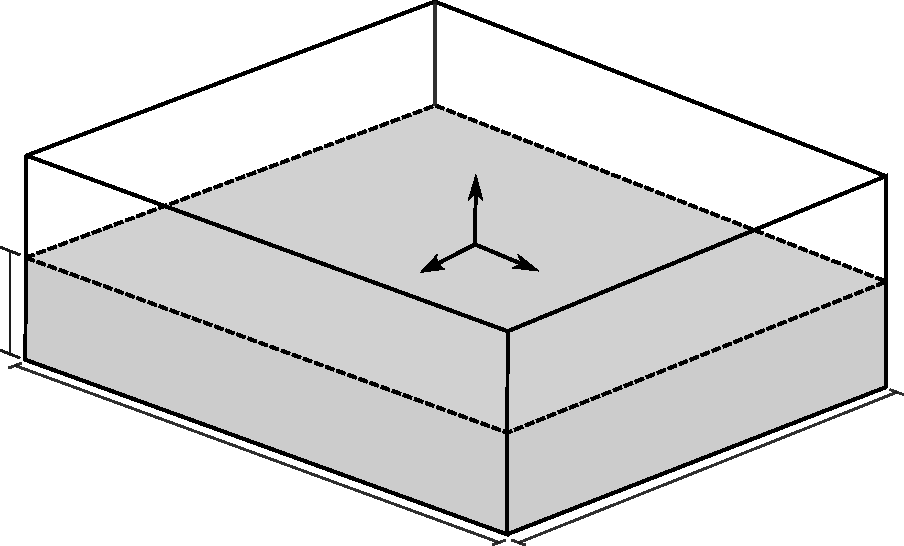
\includegraphics[width=0.44\linewidth]{figures/model.pdf}};
		\node (y) at (0.8,0.2) {$y$};
		\node [left of=y, xshift=-0.1cm] {$x$};
		\node at (0.25,0.95) {$z$};
		\node at (0.2,-0.03) {$\mathrm{O}$};
		
%		\node (h1) at (-3.9,0.7) {$h_1$};
		\node (h1) at (-3.9,0.7) {};
		\node [below of=h1, yshift=1mm, xshift=-1.1mm] {$h$};
		
		\node (Lx) at (-1.7,-1.85) {$L_y$};
		\node (Ly) at (2.5,-1.95) {$L_x$};
		
%		\node (o1) at (-1.5,-0.15) [rotate=-19] 
%		{$\Omega_1 (\rho_1, \nu_1, \sigma_1)$};
		\node (o1) at (-1.5,-0.15) {};
		\node [below of=o1, yshift=1mm, rotate=-19] 
		{$\Omega (\rho, \nu, \sigma)$};
		\node at (2,-1) {$\mathcal S$};
		
		\node at (-3.5,1.8) {(a)};
		\end{scope}
		
		\begin{scope}[xshift=8cm]
		\node (pic1) at (0,0) {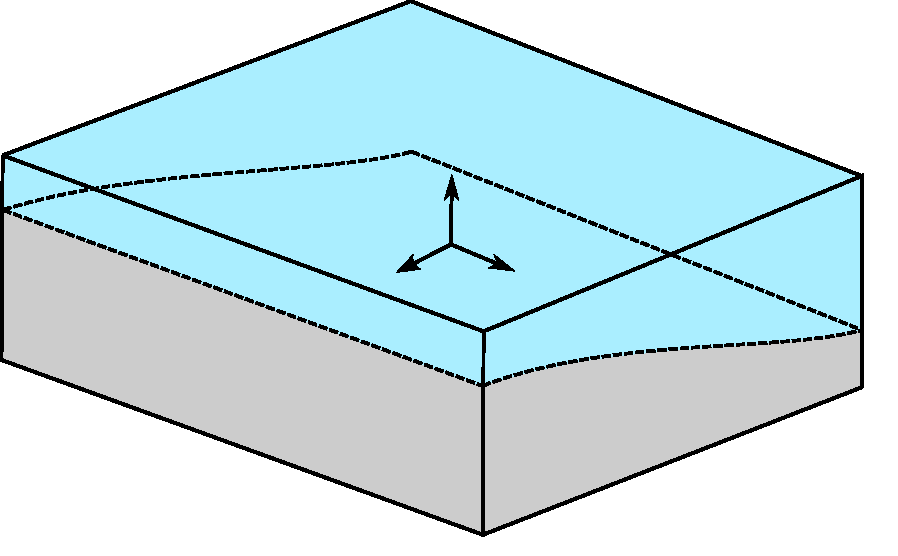
\includegraphics[width=0.4\linewidth]{figures/model_destablize.pdf}};
		\node (y) at (0.7,0.2) {$y$};
		\node [left of=y, xshift=0cm] {$x$};
		\node at (0,0.7) {$z$};
		\node at (0.17,-0.05) {$\mathrm{O}$};
		
		
		
		
		\draw[-Stealth, very thick] (3.9,-1.6) -- (3.9,1.75) node [above] {$B_z$};
		\draw[-Stealth, very thick] (4.2,1.75) -- (4.2,-1.6) node [below] {$g$};
		
		\draw [-Stealth, very thick] (-2.4,-0.62) node 
		[below, xshift=9mm, yshift=-3.5mm, rotate=-22] {$\h U \times B_z\h e_z$} -- (-0.4,-1.4) ;
		\draw [-Stealth, very thick] (2.8,-0.75) node 
		[below, xshift=-8mm, yshift=-3.5mm, rotate=23] {$\h U$} -- (0.8,-1.53) ;
		
		 \node at (-3.5,1.8) {(b)};
		 
%		\draw[lightgray,step=0.5] (pic1.south west) grid (pic1.north east);
%		
%		% Axes' labels
%		\foreach \x in {-4,-3.5,...,4} { \node [below] at (\x,0) {\x}; }
%		\foreach \y in {-2.5,-2,...,2.5} { \node [left] at (0,\y) {\y};}
%				
		\end{scope}
	\end{tikzpicture}
	\caption{The three-dimensional sketch describing the a) single-layer system $\Omega$ of depth $h$, with density, kinematic viscosity and electrical conductivity denoted as $\rho$, $\nu$ and $\sigma$ respectively, and b) the mechanism of induction ($\propto \h U \times B_z \h e_z$) due to the motion of the free surface $\mathcal{S}$ in the presence of a vertical magnetic field, $B_z$. The acceleration due to gravity $g$ acts in the downward direction along $z$-axis. }
	\label{fig:model}
\end{figure}
%%%%%%%%%%%%%% 
We consider a single layer of electrically conducting liquid $\Omega$ with density $\rho$, kinematic viscosity $\nu$, and electrical conductivity $\sigma$, confined within a rectangular domain of length $L_x$, width $L_y$, and finite depth $h$, as illustrated in Fig.\,\subref{fig:model}{a}. The undisturbed free surface $\mathcal{S}$ is located at $z=0$, while the bottom wall is located at $z=-h$. A uniform and stationary magnetic field 
\begin{equation}
	 \h B_0 = B_z \h e_z 
\end{equation} 
is applied in the vertical direction. The motion of the electrically conducting liquid in the imposed magnetic field generates the motional electromotive term $\h u\times\h B_0$, a key contributor to Ohmic dissipation. In the simple magnetohydrodynamic case of unbounded geometries or electrically conducting walls, the motional term is sufficient to determine the induced electric currents. However, in many practically relevant configurations with insulating or mixed conducting-insulating boundaries, the electric-potential contribution provides an additional component of the current density and redistributes the induced currents in accordance with charge conservation and the electrical boundary conditions.
Accordingly, the induced current density is generally given by Ohm's law
\begin{equation}
	 \h J = \sigma\left(-\bm\nabla\Psi+\h u\times\h B_0\right), \label{eq:gov_quasi_mhd} 
 \end{equation} 
 where $\Psi$ denotes the induced electric potential. Conservation of electric charge further requires
 \begin{equation} 
 \bm\nabla\cdot\h J=0. \label{eq:gov_charge_cont}
 \end{equation}
Together with the electrical boundary conditions, Eqs.\,\eqref{eq:gov_quasi_mhd} and \eqref{eq:gov_charge_cont} determine the paths along which the induced currents close within the fluid or through electrically conducting boundaries.
Taking the divergence of Eq.\,\eqref{eq:gov_quasi_mhd} and using Eq.\,\eqref{eq:gov_charge_cont} yields 
\begin{equation} 
\nabla^2\Psi = \bm\nabla\cdot \left(\h u\times\h B_0\right) = \h B_0\cdot \left(\bm\nabla\times\h u\right) - \h u\cdot \left(\bm\nabla\times\h B_0\right).
\end{equation} 
For our present wave problem, the right-hand side vanishes. The imposed magnetic field $\h B_0=B_z\h e_z$ is spatially uniform, and the leading-order gravity-wave flow is irrotational, $\bm\nabla\times\h u=0$. Consequently, the induced electric potential satisfies Laplace's equation, 
\begin{equation}
	\nabla^2\Psi=0. \label{eq:laplacian_psi} 
\end{equation} 
Although Eq.\,\eqref{eq:laplacian_psi} contains no volumetric source term, the electric potential is in general non-zero. Its spatial distribution is determined by the electrical boundary conditions and redistributes the induced currents when they cannot close freely through the surrounding walls. The solution of Eq.\,\eqref{eq:laplacian_psi} for the different conducting, insulating, and mixed boundary configurations is presented in Sec.\,\ref{sec:elec_potential}.

We now turn to the hydrodynamic problem that provides the velocity field driving the electromagnetic response. The linearized momentum and continuity equations are \begin{subequations} 
\begin{align} 
\rho\partial_t\h u + \bm\nabla p &= \h J\times B_z\h e_z +\rho\nu\nabla^2\h u, \label{eq:gov_momentum} \\ 
\bm\nabla\cdot\h u &=0. \label{eq:gov_cont} 
\end{align} 
\end{subequations} 
Here, $\h J\times B_z\h e_z$ denotes the Lorentz force associated with the induced currents. In the present formulation, the magnetic damping is treated as a perturbation to the underlying gravity-wave motion. The velocity field required to determine the induced currents can therefore be obtained from the corresponding undamped gravity-wave solution. Viscous effects in the bulk fluid are likewise neglected. For the linear sloshing modes considered here, viscous dissipation is associated predominantly with the oscillatory Stokes boundary layers at the rigid walls. These contributions have been treated in our previous work \citet{Hegde2026} and are not reconsidered in the present analysis. Outside these thin boundary layers, the wave motion is therefore taken to be inviscid and irrotational. Introducing the velocity potential $\phi$, 
\begin{equation} 
\h u=\bm\nabla\phi, 
\end{equation} 
the continuity equation \eqref{eq:gov_cont} yields, analogous to the electric potential problem, a Laplace equation for the velocity potential,
\begin{equation} 
\nabla^2\phi=0. \label{eq:laplacian_phi} 
\end{equation}
The velocity potential is subject to the impermeability condition at the rigid boundaries, 
\begin{equation} 
\bm\nabla\phi\cdot\h n=0, \label{eq:wave_no_penetration} 
\end{equation} 
where $\h n$ denotes the outward normal vector. At the undisturbed free surface $z=0$, the linearized kinematic boundary condition relates the surface displacement $\eta$ to the vertical fluid velocity, 
\begin{equation} 
\partial_t\eta = \left.\partial_z\phi\right|_{z=0}. \label{eq:free_surface_kinematic} 
\end{equation} 
The corresponding dynamic boundary condition follows from the linearized unsteady Bernoulli equation. With constant atmospheric pressure at the free surface and neglecting surface tension, it becomes 
\begin{equation} 
\left.\partial_t\phi\right|_{z=0} + g\eta = 0. \label{eq:free_surface_dynamic} \end{equation} 
For a standing gravity wave with mode indices $(m,n)$, the classic solution of the Laplace problem together with the rigid-wall and free-surface boundary conditions can be represented as
\begin{equation}
	\eta (x,y,t) = \ii i A_{mn}
	\cos{\biggl[ \frac{m\pi}{L_x}
		\biggl(x + \frac{L_x}{2}\biggr) \biggr]}
	\cos{\biggl[ \frac{n\pi}{L_y}
		\biggl(y + \frac{L_y}{2}\biggr) \biggr]}
	\ii{e}^{\ii i\omega t},
	\label{eq:eta}
\end{equation}
for the free-surface displacement, and
\begin{equation}
	\phi = -A_{mn}
	\frac{\omega}{k}
	\frac{\cosh{[k\bigl(z + h \bigr)]}}{\sinh{[kh]}}
	\cos{\biggl[ \frac{m\pi}{L_x}
		\biggl(x + \frac{L_x}{2}\biggr) \biggr]}
	\cos{\biggl[ \frac{n\pi}{L_y}
		\biggl(y + \frac{L_y}{2}\biggr) \biggr]}
	\ii{e}^{\ii i\omega t},
	\label{eq:vel_potential}
\end{equation}
for the corresponding velocity potential. Here, $A_{mn}$ denote the mode-dependent wave amplitudes and $m,n\in\mathbb{N}_0$ with $(m,n)\neq(0,0)$ are the mode indices, specifying the number of half wavelengths in the $x$ and $y$ directions, respectively.
The wavenumber associated with the mode $(m,n)$ must satisfy
\begin{equation}
	k = \pi\sqrt{
		\left(\frac{m}{L_x}\right)^2
		+
		\left(\frac{n}{L_y}\right)^2
	}.
	\label{eq:wavenumber}
\end{equation}
The eigenfrequencies of the wave modes follow from the linear free-surface boundary conditions and satisfies the finite-depth gravity-wave dispersion relation
\begin{equation}
	\omega = \pm\sqrt{gk\tanh(kh)}.
	\label{eq:ang_freq}
\end{equation}
The resulting velocity field $\h u=\bm\nabla\phi$ constitutes the hydrodynamic basis for the subsequent calculation of the induced electric potential, current distribution, and Ohmic dissipation.
 
The present formulation is restricted to linear, small-amplitude gravity waves. Consistent with the perturbative treatment of the magnetic field, both magnetic induction and Lorentz-force feedback are assumed to remain weak, requiring the magnetic Reynolds number $\ii{Rm}$ and the interaction parameter $N$ (Stuart number) to be small
\begin{equation}
	\ii{Rm}
	=
	\mu_0\sigma\omega L^2
	\ll 1,
	\qquad
	N
	=
	\frac{\sigma B_z^2}{\rho\omega}
	< 1,
	\label{eq:mag_parameters}
\end{equation}
where $\mu_0$ is the permeability of free space, $L\sim\sqrt{L_x L_y}$ is the characteristic length scale, and the characteristic velocity of the wave motion is taken as $U\sim\omega L$. With these characteristic scales, $\ii{Rm}\ll1$ justifies the quasi-static approximation, such that the magnetic field induced by the wave motion is negligible compared with the imposed field $\h B_0$. The condition $N\ll1$ ensures that the Lorentz-force feedback remains a perturbation to the leading-order gravity-wave dynamics. Consequently, rotational corrections to the potential solutions induced by the Lorentz force are neglected, while its dissipative effect on the wave is retained.
Finally, we introduce the Hartmann number to quantify the relative importance of electromagnetic and viscous effects,
\begin{equation}
	\ii{Ha}
	=
	B_z L
	\sqrt{\frac{\sigma}{\rho\nu}},
	\label{eq:hartmann_number}
\end{equation}
which is particularly relevant to estimate the magnetic modification of the viscous boundary layers, including the formation of Hartmann and Shercliff layers, see Sec.\,\ref{sec:hartmann_and_shercliff}.
 


\subsection{Calculation of electric potentials}
\label{sec:elec_potential}


\begin{table}%[H] add [H] placement to break table across pages
	\caption{The four different cases adopted in the current study and its respective boundary conditions. The conducting walls are highlighted in orange while the insulating walls are in white. The free surface is marked in red.}
	\label{tab:table_sim}
	\begin{ruledtabular}
		\begin{tabular}{llll}
			Case No. &  Case name & \multicolumn{2}{l}{Boundary conditions} 
			\\  \hline 
			 &	 &
			\multirow{5}{*}{
				\begin{tikzpicture}
					\node at (0,0) {
						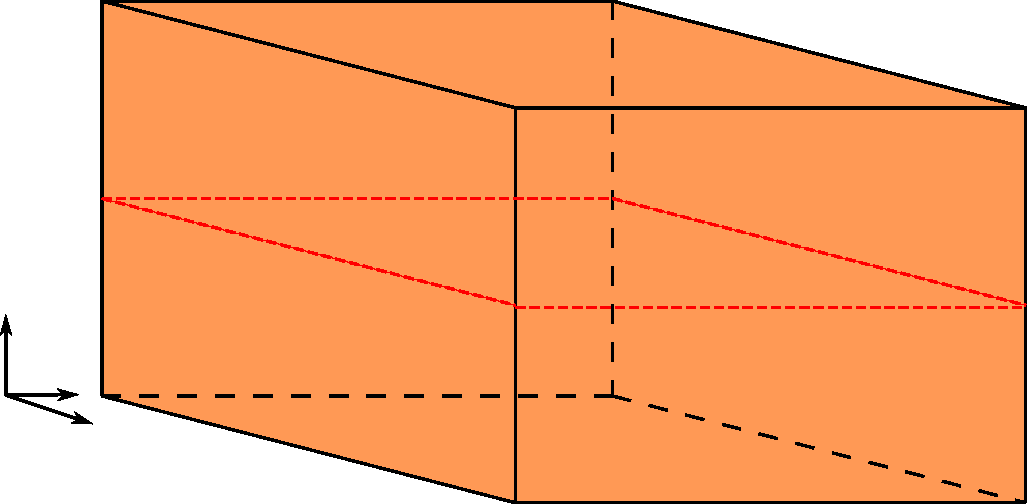
\includegraphics[width=0.3\textwidth]{figures/BC_case1.pdf}
					};
					\node (y) at(-2.1,-0.95) {$y$};
					\node (x) [above of=y, xshift=-0.2cm, yshift=-0.6cm] {$x$};
					\node (z) [above of=y, xshift=-0.55cm, yshift=-0.2cm] {$z$};
				\end{tikzpicture} 
			}
			& 
			\\
			1 & B.C 1 & & 
			\\
			& & & $\Psi\bigl|_{x=\pm 0.5L_x}=\Psi\bigl|_{y=\pm 0.5L_y}=0$,
			\\
			& & & 
			\\
			& & & $\Psi|_{z=-h} = 0$, $\partial_z\Psi|_{z=0} = 0$.
			\\[25pt] \hline
			
			 &  &
			\multirow{5}{*}{
				\begin{tikzpicture}
					\node at (0,0) {
						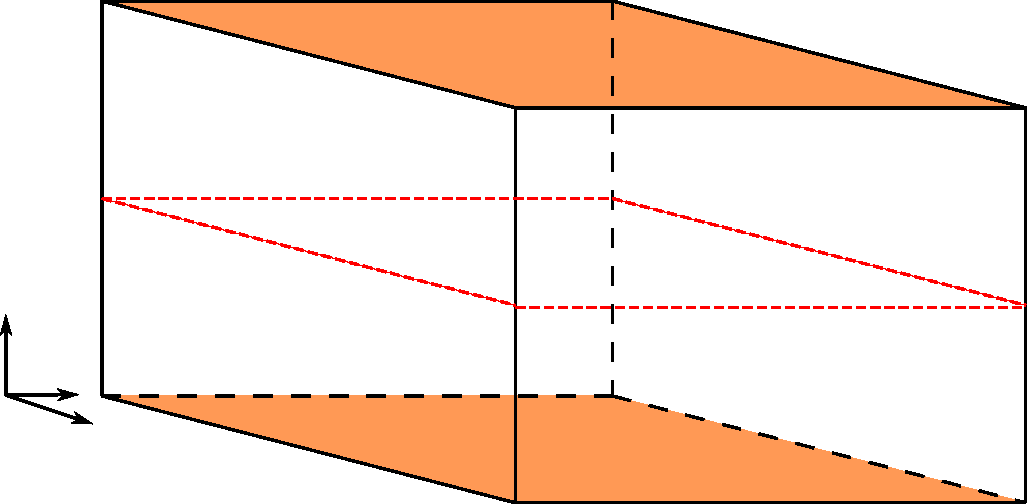
\includegraphics[width=0.3\textwidth]{figures/BC_case2.pdf}
					};
					\node (y) at(-2.1,-0.95) {$y$};
					\node (x) [above of=y, xshift=-0.2cm, yshift=-0.6cm] {$x$};
					\node (z) [above of=y, xshift=-0.55cm, yshift=-0.2cm] {$z$};
				\end{tikzpicture}
			}
			& 
			\\
			2 & B.C 2 & & $\Psi\bigl|_{x=\pm 0.5L_x}=0$, 
			\\
			& & & 
			\\
			& & & $\partial_y \Psi\bigl|_{y=\pm 0.5L_y}= -\partial_x\phi B_z$,
			\\
			& & & 
			\\
			& & & $\partial_z\Psi|_{z=0} = 0$, $\partial_z\Psi|_{z=-h} = 0$.
			\\[14pt] \hline
			% 		
			 &	  &
			\multirow{5}{*}{
				\begin{tikzpicture}
					\node at (0,0) {
						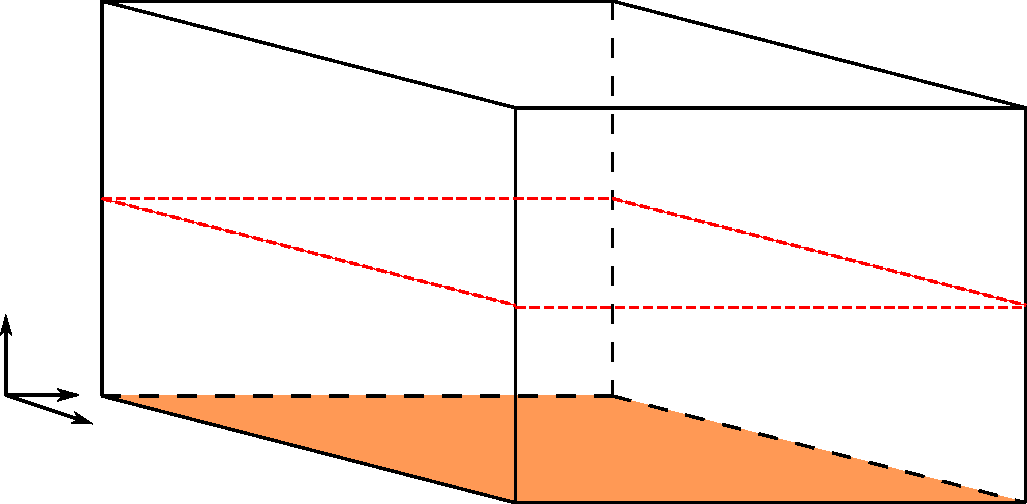
\includegraphics[width=0.3\textwidth]{figures/BC_case3.pdf}
					};
					\node (y) at(-2.1,-0.95) {$y$};
					\node (x) [above of=y, xshift=-0.2cm, yshift=-0.6cm] {$x$};
					\node (z) [above of=y, xshift=-0.55cm, yshift=-0.2cm] {$z$};
				\end{tikzpicture}
			}
			& 
			\\
			3 & B.C 3 & & $\partial_x \Psi\bigl|_{x=\pm 0.5L_x} = \partial_y\phi B_z$, 
			\\
			& & & 
			\\
			& & & $\partial_y \Psi\bigl|_{y=\pm 0.5L_y}= -\partial_x\phi B_z$,
			\\
			& & & 
			\\
			& & & $\partial_z\Psi|_{z=0} = 0$, $\Psi|_{z=-h} = 0$.
			\\[14pt] \hline
			
			 &  &
			\multirow{5}{*}{
				\begin{tikzpicture}
					\node at (0,0) {
						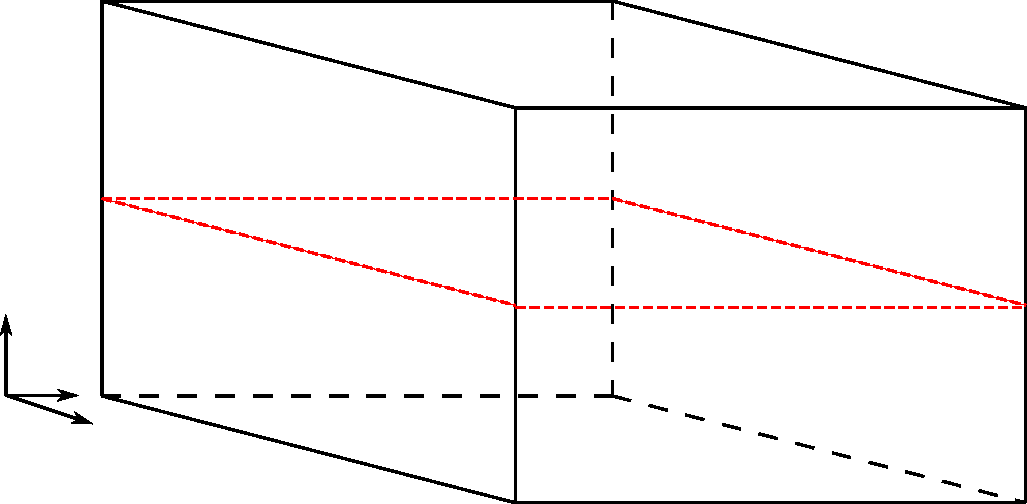
\includegraphics[width=0.3\textwidth]{figures/BC_case4.pdf}
					};
					\node (y) at(-2.1,-0.95) {$y$};
					\node (x) [above of=y, xshift=-0.2cm, yshift=-0.6cm] {$x$};
					\node (z) [above of=y, xshift=-0.55cm, yshift=-0.2cm] {$z$};
				\end{tikzpicture}
			}
			&
			\\
			4 & B.C 4 & & $\partial_x \Psi\bigl|_{x=\pm 0.5L_x} = \partial_y\phi B_z$, 
			\\
			& & & 
			\\
			& & & $\partial_y \Psi\bigl|_{y=\pm 0.5L_y}= -\partial_x\phi B_z$,
			\\
			& & & 
			\\
			& & & $\partial_z\Psi|_{z=0} = 0$, $\partial_z\Psi|_{z=-h} = 0$.
			\\[14pt]
		\end{tabular}
	\end{ruledtabular}
\end{table}

The electric potential $\Psi$ entering Ohm's law is obtained from the Laplace equation \eqref{eq:laplacian_psi}, subject to the electrical boundary conditions at the surrounding walls. These boundary conditions determine the spatial distribution of $\Psi$ and, consequently, the redistribution and closure of the induced currents. Since the relevant electrical boundary conditions depend on the particular physical or industrial configuration, we consider four idealized cases, denoted B.C 1--B.C 4 and summarized in Table\,\ref{tab:table_sim}. In B.C 1, all bounding walls are perfect electrical conductors and act as ideal electrodes ($\Psi|_{\rm wall}=0)$.
In B.C 2, the pair of sidewalls normal to the $x$-axis is perfectly conducting, whereas the remaining walls are perfect electrical insulators. At the insulating boundaries, current penetration is prohibited by the no-outflow condition
\begin{equation}
	\h J\cdot\h n|_{\rm wall}=0.
\end{equation}
In B.C 3, the bottom wall is perfectly conducting, while all sidewalls are perfect electrical insulators. Finally, B.C 4 corresponds to a fully insulating configuration. B.C 1 constitutes the trivial solution of the electric-potential problem. Since the potential in the fluid is constrained by the conducting boundaries, Eq.\,\eqref{eq:laplacian_psi} gives 
\begin{align}
\Psi(\ii{B.C 1})=0
\end{align}
throughout $\Omega$ \cite{Sreenivasan2005}. In this case, the electrical properties of the bottom wall are inconsequential because the induced currents are purely horizontal and close through the conducting vertical sidewalls. By contrast, for B.C 2--B.C 4, the no-current-outflow conditions at the insulating boundaries determine the non-trivial electric-potential distributions and thereby the corresponding current-closure paths.
Details of the solutions to these boundary-value problems are provided in Sec.\,I of the Supplemental Material \cite{SMmagdamp_hegde}. The resulting electric potentials for the four boundary configurations are given below. 
\\
\indent First, for B.C 2:
\begin{gather}
	\Psi (\ii{B.C 2})= 
	\sum_{a,b=0}^{\infty}
	\grave{\mathcal{B}}_{ab} 
	\left(
	\frac{1-(-1)^n}{2\sech{[\grave\xi_y y]}} + \frac{1+(-1)^n}{2\csch{[\grave\xi_y y]}}
	\right)
	\sin{\biggl[ \frac{a\pi}{L_x}\biggl(x + \frac{L_x}{2}\biggr)\biggr]}
	\cos{\biggl[ \frac{b\pi}{h}\bigl(z + h\bigr)\biggr]}
	.
	\label{eq:bc2_potential_old}
\end{gather}
Here, only the insulating pair of sidewalls normal to the $y$-axis, the bottom wall and free surface contribute to the electric potential. The contribution from the non-shallow depth $h$ adds an additional sum to the solution that is absent in the shallow limit \cite{Sreenivasan2005}. The hyperbolic functions alternate based on the parity of the wave mode $n$. The sine and cosine terms are attributed to the conducting pair of sidewalls and the insulating boundaries at the bottom and the free surface, respectively. The coefficient $\grave{\mathcal{B}}_{ab}$ is non-zero only for the the condition $a=m$ and the potential $\Psi (\ii{B.C 2})=0$ when $m=0$. Therefore, Eq.\,\eqref{eq:bc2_potential_old} simplifies to
\begin{gather}
	\Psi (\ii{B.C 2})= 
	\sum_{b=0}^{\infty}
	\grave{\mathcal{B}}_{mb} 
	\left(
	\frac{1-(-1)^n}{2\sech{[\grave\xi_y y]}} + \frac{1+(-1)^n}{2\csch{[\grave\xi_y y]}}
	\right)
	\sin{\biggl[ \frac{m\pi}{L_x}\biggl(x + \frac{L_x}{2}\biggr)\biggr]}
	\cos{\biggl[ \frac{b\pi}{h}\bigl(z + h\bigr)\biggr]}
	,
	\label{eq:bc2_potential_new}
	\intertext{where,}
	\grave\xi_y = \pi\sqrt{\frac{m^2}{L_x^2} + \frac{b^2}{h^2} }, \quad 
	\grave{\mathcal{B}}_{mb}
	= 
	\frac{-2A_{mn}\:\omega B_z m \pi (-1)^{n+b}}
	{\epsilon_{b}\:\grave\xi_y L_x 
		\left(
		\dfrac{1-(-1)^n}{2\csch{[0.5\grave\xi_y L_y]}} + \dfrac{1+(-1)^n}{2\sech{[0.5\grave\xi_y L_y]}}
		\right)
	}
	\frac{h}{(k^2h^2 + b^2\pi^2)},
	\quad \epsilon_r = \left\{
	\begin{array}{cc}
		2, & r=0 \\
		1, & r\neq 0
	\end{array}
	\right . .
	\label{eq:bc2_B}
\end{gather}
\indent Second, for B.C 3: 
\begin{align}
	\nn
	\Psi (\ii{B.C 3})&= 
	\sin{[(z+h)p_h]} \left(
	\dfrac{ \tilde{\mathcal A_0} \bigl((-1)^{m} - (-1)^n \bigr)\:
		\sinh{[p_h x]}}{2p_h \cosh{[0.5p_hL_x]}} 
	- 
	\dfrac{
	\tilde{\mathcal A_0} \bigl((-1)^{m} + (-1)^n \bigr) \:
		\cosh{[p_h x]}}{2p_h \sinh{[0.5p_hL_x]}}
	\right.
	\\
	\nn
	&+
	\left.
	\dfrac{ \tilde{\mathcal B_0} \bigl((-1)^{n} - (-1)^m \bigr)\:
		\sinh{[p_h y]}}{2p_h \cosh{[0.5p_hL_y]}} 
	- 
	\dfrac{
		\tilde{\mathcal B_0} \bigl((-1)^{n} + (-1)^m \bigr) \:
		\cosh{[p_h y]}}{2p_h \sinh{[0.5p_hL_y]}}
	\right)
	\\
	\nn
	&+
	\sum_{\substack{a, b \geq 0 \\ 
			(a,b)\neq (0,0) \\
			a\neq n}
		}^{\infty}
	\tilde{\mathcal{A}}_{ab}
	\left(
	\frac{1-(-1)^m}{2\sech{\bigl[\tilde\xi_x x \bigr]}} + \frac{1+(-1)^m}{2\csch{\bigl[\tilde\xi_x x \bigr]}}
	\right)
	\cos{\biggl[ \frac{a\pi}{L_y}\biggl(y + \frac{L_y}{2}\biggr)\biggr]}
	\sin{\biggl[ (2b+1)p_h\bigl(z + h\bigr)\biggr]} 
	\\
	&+
	\sum_{\substack{a, b \geq 0 \\ (a,b) 
			\neq (0,0)\\
			a\neq m		
	}}^{\infty}
	\tilde{\mathcal B}_{ab}
	\left(
	\frac{1-(-1)^n}{2\sech{\bigl[\tilde\xi_y y\bigr]}} + \frac{1+(-1)^n}{2\csch{\bigl[\tilde\xi_y y\bigr]}}
	\right)
	\cos{\biggl[ \frac{a\pi}{L_x}\biggl(x + \frac{L_x}{2}\biggr)\biggr]}
	\sin{\biggl[ (2b+1)p_h\bigl(z + h\bigr)\biggr]}
	,
	\label{eq:bc3_potential}
\end{align}
with coefficients,
\begin{align}
	p_h = \frac{\pi}{2h},\quad
	\tilde\xi_x = \pi\sqrt{\frac{a^2}{L_y^2} + \frac{(1+2b)^2}{4h^2} }, \quad
	\tilde\xi_y = \pi\sqrt{\frac{a^2}{L_x^2} + \frac{(1+2b)^2}{4h^2} }, 
	\quad \epsilon_r = \left\{
	\begin{array}{cc}
		2, & r=0 \\
		1, & r\neq 0
	\end{array}
	\right . ,
	\label{eq:bc3_xi}
\end{align}
\begin{align}
	\tilde{\mathcal A_0} &= 
	\frac{
		-4A_{mn}\omega B_z \bigl( (-1)^{m+1} + (-1)^{m+n} \bigr) }
	{k L_y}
	\dfrac{(2kh + \pi\csch{[kh]})}{4k^2h^2 + \pi^2}
	, 
	\label{eq:bc3_constantsA0}
	\\
	\tilde{\mathcal B_0} &= 
	\frac{
		4A_{mn} \omega B_z \bigl( (-1)^{n+1} + (-1)^{m+n} \bigr) }
	{k L_x}
	\dfrac{(2kh + \pi\csch{[kh]})}{4k^2h^2 + \pi^2}
	,
	\label{eq:bc3_constantsB0}
\end{align}
\begin{align}
	\tilde{\mathcal A}_{ab} & =  
	\frac{8A_{mn} \: \omega B_z n^2 \bigl( (-1)^{m+1} + (-1)^{a+m+n} \bigr)
	}
	{\epsilon_a \: (a^2-n^2)
	\left(
	\dfrac{1-(-1)^m}{2\csch{\bigl[0.5\tilde\xi_x L_x \bigr]}} + 
	\dfrac{1+(-1)^m}{2\sech{\bigl[0.5\tilde\xi_x L_x \bigr]}}
	\right)\tilde\xi_x L_y k
	}
	\frac{\left(
		2kh (-1)^b + (1+2b)\pi\csch{[kh]}
		\right)}
	{(4k^2h^2 + (1+2b)^2\pi^2)},
	\label{eq:bc3_A}
	\\
%\end{align}
%\begin{align}
	\tilde{\mathcal B}_{ab} &= 
	\frac{-8A_{mn} \: \omega B_z m^2 \bigl( (-1)^{n+1} + (-1)^{a+m+n} \bigr)
	}
	{\epsilon_a \: (a^2-m^2)
		\left(
		\dfrac{1-(-1)^n}{2\csch{\bigl[0.5\tilde\xi_y L_y \bigr]}} + 
		\dfrac{1+(-1)^n}{2\sech{\bigl[0.5\tilde\xi_y L_y \bigr]}}
		\right)\tilde\xi_y L_x k
	}
	\frac{\left(
		2kh (-1)^b + (1+2b)\pi\csch{[kh]}
		\right)}
	{(4k^2h^2 + (1+2b)^2\pi^2)}.
	\label{eq:bc3_B}
\end{align}
In Eq.\,\eqref{eq:bc3_potential}, the terms containing the coefficients $\tilde{\mathcal A}_{ab}$ and $\tilde{\mathcal B}_{ab}$ correspond to the insulating boundary conditions of the sidewalls perpendicular to the $x$- and $y$-axis accordingly. The constant terms $\tilde{\mathcal A}_0$ and $\tilde{\mathcal B}_0$ are necessary to satisfy the boundary conditions when $a,b=0$; a condition where $\tilde\xi_x=\tilde\xi_y=p_h$ and needs to be separated from the double sums to avoid indeterminate representation of $\tilde{\mathcal A}_{ab}$ and $\tilde{\mathcal B}_{ab}$.
\\
\indent Lastly, for B.C 4:
\begin{align}
	\nn
	\Psi (\ii{B.C 4})&= 
	\ddot{\mathcal A}_0x - \frac{\ddot{\mathcal A}_0 \bigl( (-1)^n + (-1)^{m+n+1} \bigr) }{2L_x}
	\left(x- \frac{L_x}{2}\right)^2
	+
	\ddot{\mathcal B}_0y - \frac{\ddot{\mathcal B}_0 \bigl( (-1)^m + (-1)^{m+n+1} \bigr) }{2L_y}
	\left(y- \frac{L_y}{2}\right)^2
	\\
	\nn
	&+
	\sum_{\substack{a, b \geq 0 \\ (a,b) 
			\neq (0,0) \\
		a\neq n	
	}}^{\infty}
	\ddot{\mathcal A}_{ab} 
	\left(
	\frac{1-(-1)^m}{2\sech{\bigl[ \ddot\xi_x x \bigr]}} + \frac{1+(-1)^m}{2\csch{\bigl[ \ddot\xi_x x \bigr]}}
	\right)
	\cos{\biggl[ \frac{a\pi}{L_y}\biggl(y + \frac{L_y}{2}\biggr)\biggr]}
	\cos{\biggl[ \frac{b\pi}{h}\bigl(z +  h\bigr)\biggr]} 
	\\
	&+
	\sum_{\substack{a, b \geq 0 \\ (a,b) 
			\neq (0,0) \\
			a\neq m	
	}}^{\infty}
	\ddot{\mathcal B}_{ab} 
	\left(
	\frac{1-(-1)^n}{2\sech{\bigl[ \ddot\xi_y y \bigr]}} + \frac{1+(-1)^n}{2\csch{\bigl[ \ddot\xi_y y \bigr]}}
	\right)
	\cos{\biggl[ \frac{a\pi}{L_x}\biggl(x + \frac{L_x}{2}\biggr)\biggr]}
	\cos{\biggl[ \frac{b\pi}{h}\bigl(z +  h\bigr)\biggr]}
	,
	\label{eq:bc4_potential}
\end{align}
with coefficients,
\begin{equation}
	\ddot\xi_x = \pi\sqrt{
		\frac{a^2}{L_y^2} + \frac{b^2}{h^2}
	}
	,\quad
	\ddot\xi_y = \pi\sqrt{
		\frac{a^2}{L_x^2} + \frac{b^2}{h^2}
	},
	\quad \epsilon_r = \left\{
	\begin{array}{cc}
		2, & r=0 \\
		1, & r\neq 0
	\end{array}
	\right . ,
\end{equation}
\begin{align}
	\ddot{\mathcal A}_0 &= -A_{mn}
	\frac{
		\omega B_z \bigl( (-1)^{m+1} + (-1)^{m+n} \bigr) }
	{k^2 L_y h}, \qquad
	\ddot{\mathcal B}_0 = A_{mn}
	\frac{
		\omega B_z \bigl( (-1)^{n+1} + (-1)^{m+n} \bigr) }
	{k^2 L_x h}
	,
	\label{eq:bc4_constants}
\end{align}
\begin{align}
	\ddot{\mathcal A}_{ab} &= 
	\frac{4A_{mn}\; \omega B_z n^2 
		\bigl( (-1)^{m+b+1} + (-1)^{a+b+m+n} \bigr)}
	{\epsilon_a\epsilon_b \: (a^2 -n^2) 
		\left(
		\dfrac{1-(-1)^m}{2\csch{\bigl[0.5\ddot\xi_x L_x \bigr]}} + \dfrac{1+(-1)^m}{2\sech{\bigl[0.5\ddot\xi_x L_x \bigr]}}
		\right)
		\ddot\xi_x L_y }
	\frac{h}
	{(k^2h^2 + b^2\pi^2) },
		\label{eq:bc4_Acoeff}
	\\
	\ddot{\mathcal B}_{ab} &= 
	\frac{-4A_{mn} \; \omega B_z m^2 \bigl( (-1)^{n+b+1} + (-1)^{a+b+m+n} \bigr)}
	{\epsilon_a\epsilon_b \:  (a^2 -m^2) 
		\left(
		\dfrac{1-(-1)^n}{2\csch{\bigl[0.5\ddot\xi_y L_y \bigr]}} + \dfrac{1+(-1)^n}{2\sech{\bigl[0.5\ddot\xi_y L_y \bigr]}}
		\right)
		\ddot\xi_y L_x } 
		\frac{h}
		{(k^2h^2 + b^2\pi^2) }.
	\label{eq:bc4_Bcoeff}
\end{align}
%%%%%%%%%%%%%
The terms containing $\ddot{\mathcal A}_0$ and $\ddot{\mathcal B}_0$ are to satisfy the boundary condition when $a,b=0$ in the double sum.
\\
\indent Although Eqs.\,(\ref{eq:bc2_potential_new}, \ref{eq:bc3_potential} and \ref{eq:bc4_potential}) represent the induced electric potentials of single-layer conducting fluid systems, they can also be applied to two-layer stratified systems with large conductivity differences (eg., aluminium reduction cells, liquid metal batteries). In these systems, the interface acts like an electrically insulating wall given by the interfacial condition $\partial_z\Psi_i|_{z=0}\approx 0$, where $i=1,2$ is the index of the upper and lower layer \cite{Herreman2019}.  
%%%%%%%%%%%%%
\begin{figure}
	\begin{tikzpicture}
		\node (pic1) at (-5,0) 
		{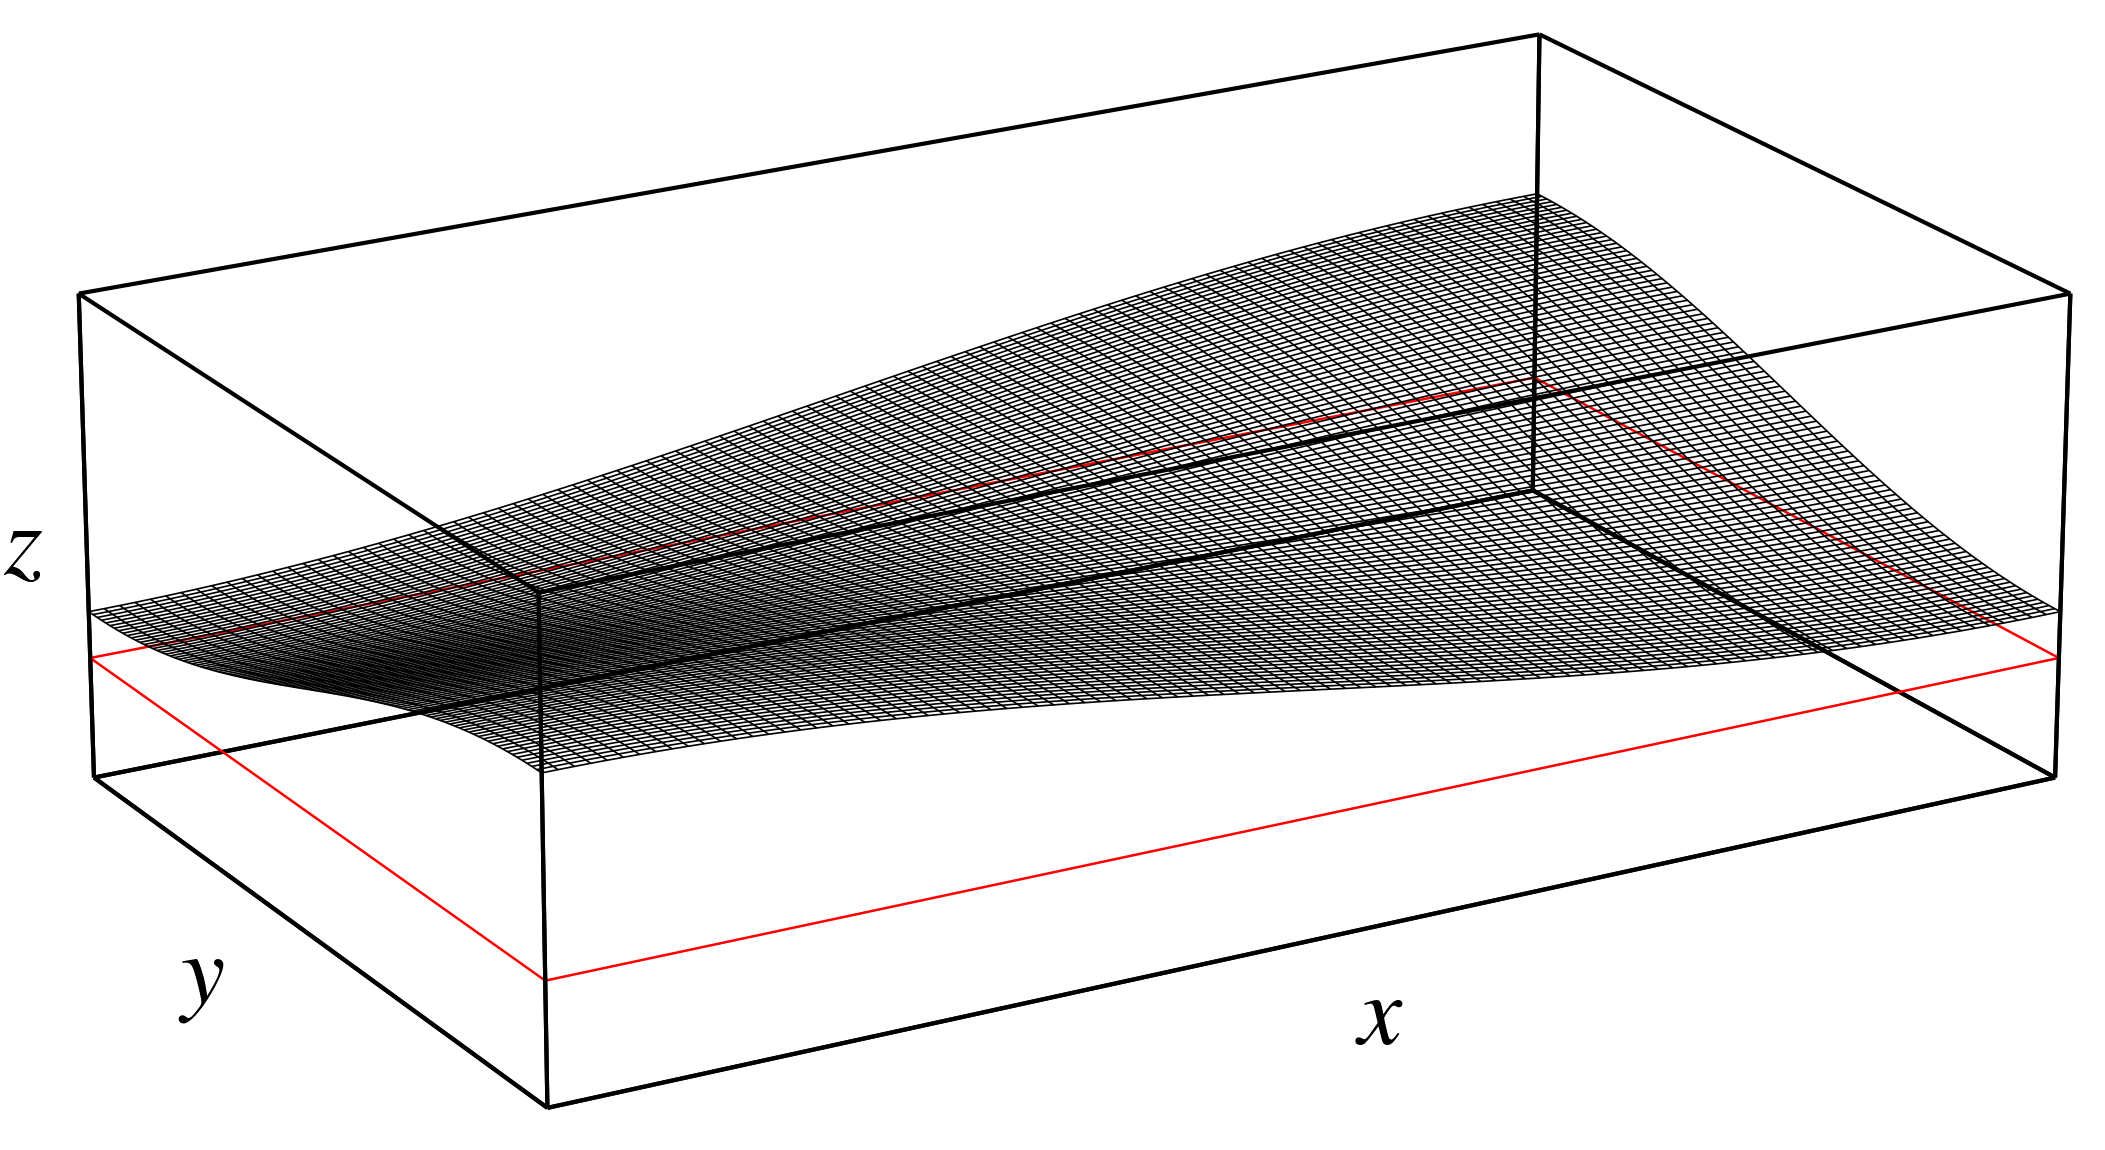
\includegraphics[width=0.45\linewidth]{figures/3-wave_1.png} };
		\node (pic2) at (3.8,0)
		{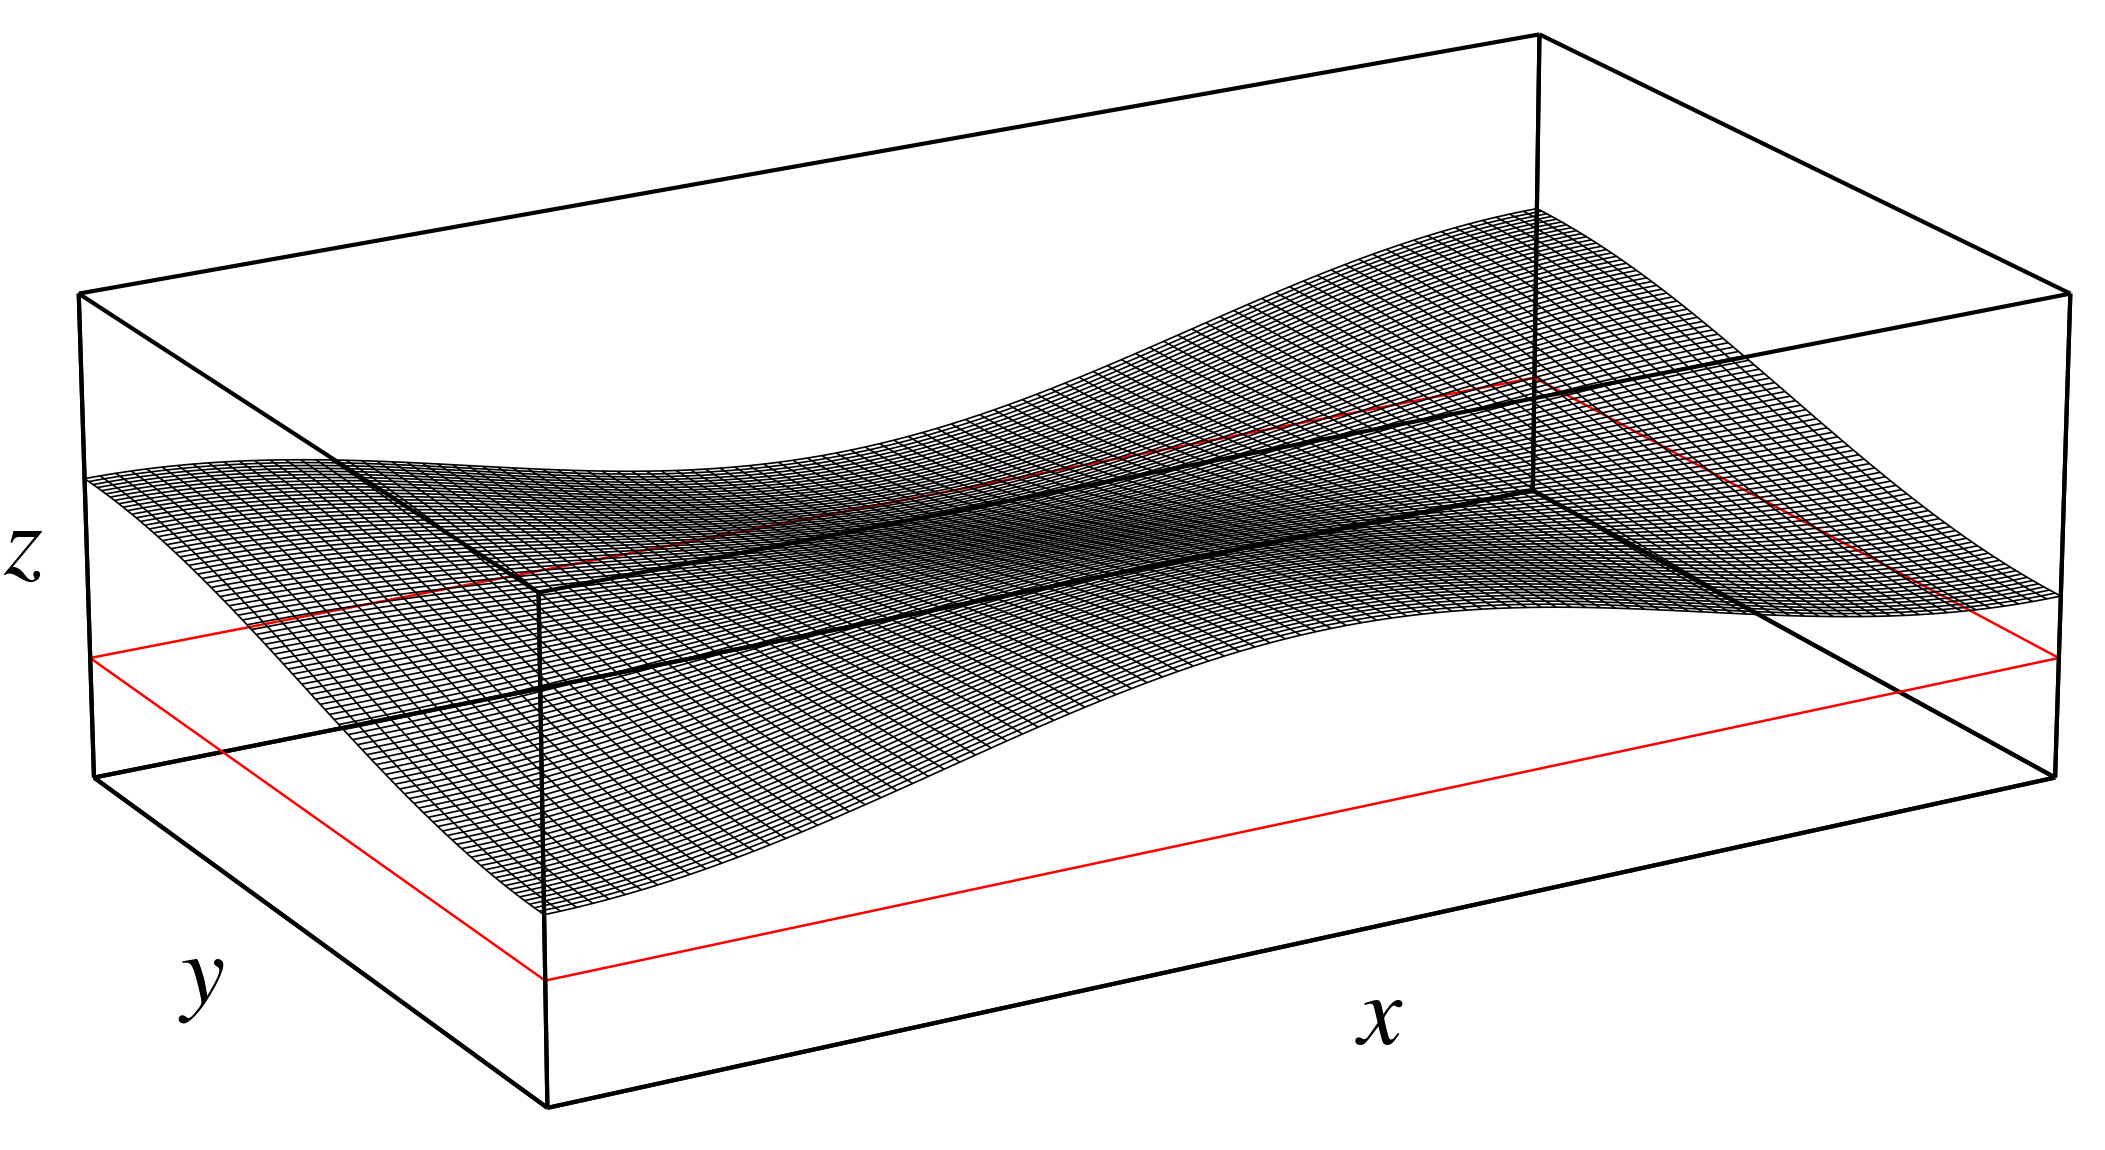
\includegraphics[width=0.45\linewidth]{figures/3-wave_0.png} };
		\node [above of=pic1, xshift=-3.9cm, yshift=0.9cm] {(a)};
		\node [above of=pic2, xshift=-3.9cm, yshift=0.9cm] {(b)};
	\end{tikzpicture}
	\caption{The free surface wave elevation for a standing wave of mode a) $(1,1)$ and b) $(2,1)$ in a rectangular domain. The horizontal cross-section of the volume is highlighted in red, and is the area of interest for the mapping of wave-induced eddy currents.}
	\label{fig:wave_modes}
\end{figure}
%%%%%%%%%%%%%
\subsection{Eddy current distribution}
\label{sec:eddy_current}
%%%%%%%%%%%%%
\begin{figure}
	\begin{tikzpicture}
		\begin{scope}
			\node (c11) at (-4.25,0) {
				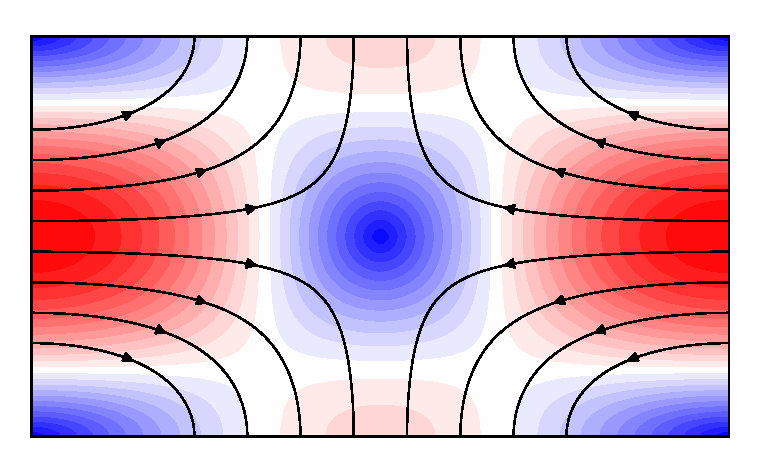
\includegraphics[width=0.45\textwidth] {figures/C1_streamline_1-1.eps}};
			\node (c12) at (4.25,0) {
				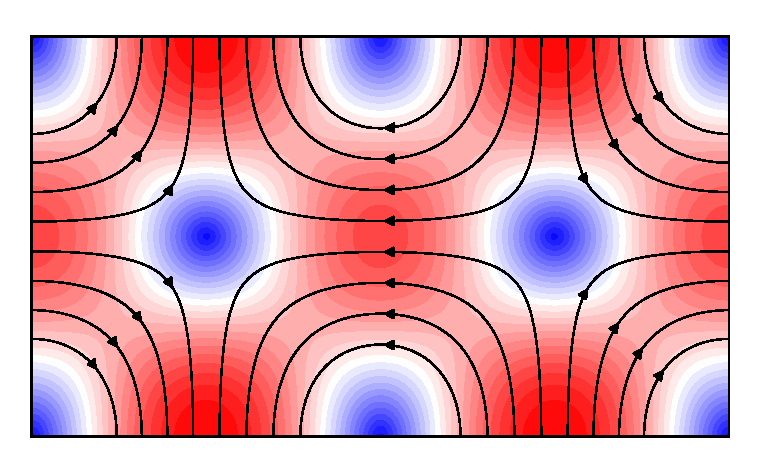
\includegraphics[width=0.45\textwidth] {figures/C1_streamline_2-1.eps}};
			\node (case) [above of=c11, xshift=-3.4cm, yshift=1.5cm] {B.C 1:};
			\node (a) [below of=case, xshift=-0.7cm, yshift=4mm] {(a)};
			\node (b) [right of=a, xshift=7.47cm] {(b)};
			
			\node [below of=c11, yshift=-1.5cm] {$x$};
			\node [left of=c11, xshift=-3cm] {$y$};
			
			\node [below of=c12, yshift=-1.5cm] {$x$};
			\node [left of=c12, xshift=-3cm] {$y$};
		\end{scope}
		\label{fig:eddy_ab}
		\begin{scope}[yshift=-5.3cm]
			\node (c11) at (-4.25,0) {
				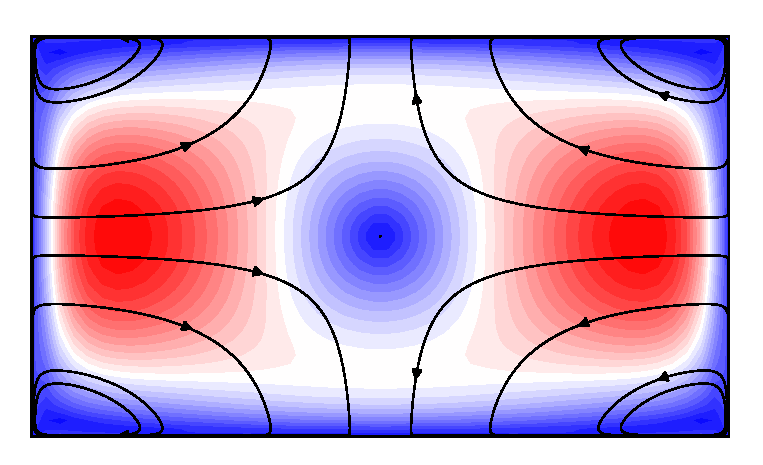
\includegraphics[width=0.45\textwidth] {figures/C2_streamline_1-1.eps}};
			\node (c12) at (4.25,0) {
				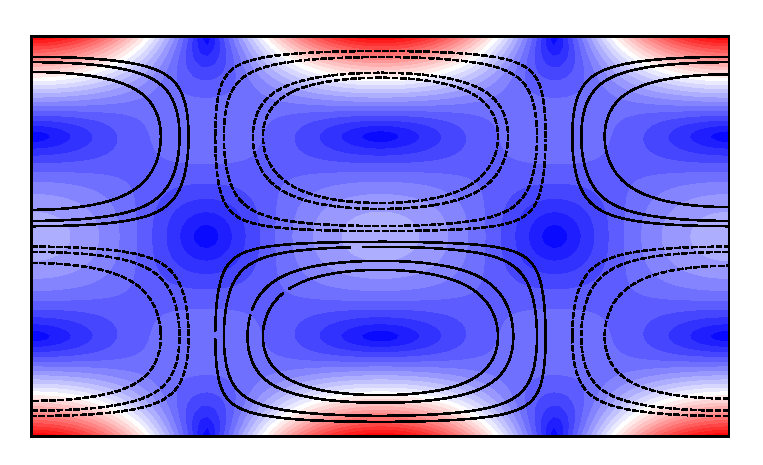
\includegraphics[width=0.45\textwidth] {figures/C2_streamline_2-1.eps}};
			\node (case) [above of=c11, xshift=-3.4cm, yshift=1.5cm] {B.C 2:};
			\node (a) [below of=case, xshift=-0.7cm, yshift=4mm] {(c)};
			\node (b) [right of=a, xshift=7.47cm] {(d)};
			
			\node [below of=c11, yshift=-1.5cm] {$x$};
			\node [left of=c11, xshift=-3cm] {$y$};
			
			\node [below of=c12, yshift=-1.5cm] {$x$};
			\node [left of=c12, xshift=-3cm] {$y$};
		\end{scope}
		\label{fig:eddy_cd}
		\begin{scope}[yshift=-10.6cm]
			\node (c11) at (-4.25,0) {
				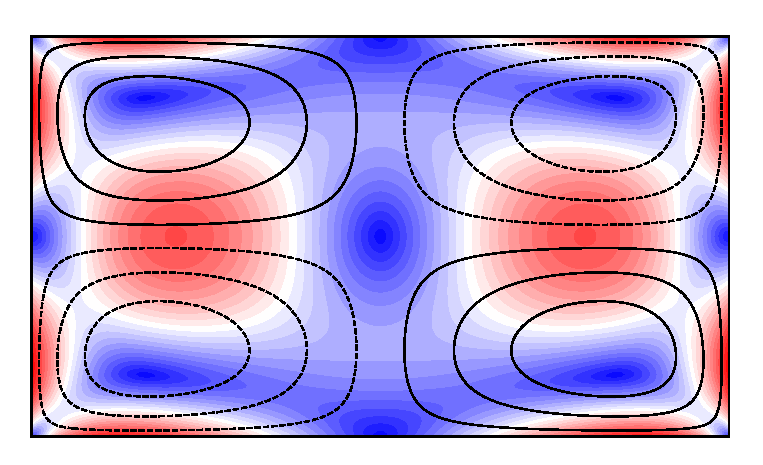
\includegraphics[width=0.45\textwidth] {figures/C3_streamline_1-1.eps}};
			\node (c12) at (4.25,0) {
				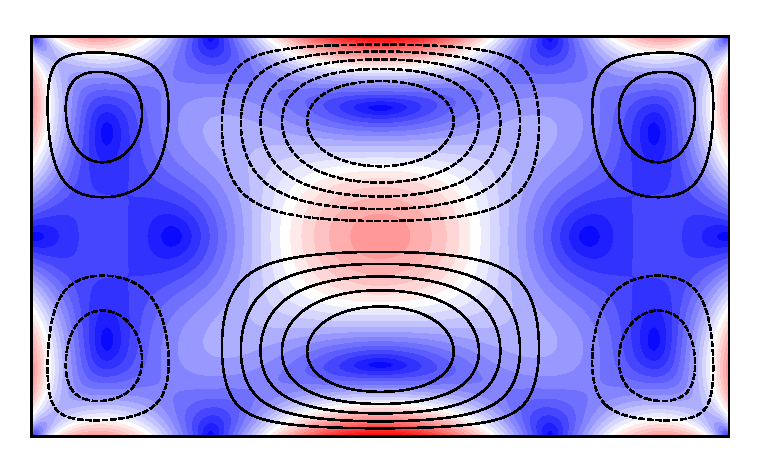
\includegraphics[width=0.45\textwidth] {figures/C3_streamline_2-1.eps}};
			\node (case) [above of=c11, xshift=-3.4cm, yshift=1.5cm] {B.C 3:};
			\node (a) [below of=case, xshift=-0.7cm, yshift=4mm] {(e)};
			\node (b) [right of=a, xshift=7.47cm] {(f)};
			
			\node [below of=c11, yshift=-1.5cm] {$x$};
			\node [left of=c11, xshift=-3cm] {$y$};
			
			\node [below of=c12, yshift=-1.5cm] {$x$};
			\node [left of=c12, xshift=-3cm] {$y$};
		\end{scope}
		\label{fig:eddy_ef}
		\begin{scope}[yshift=-15.9cm]
			\node (c11) at (-4.25,0) {
				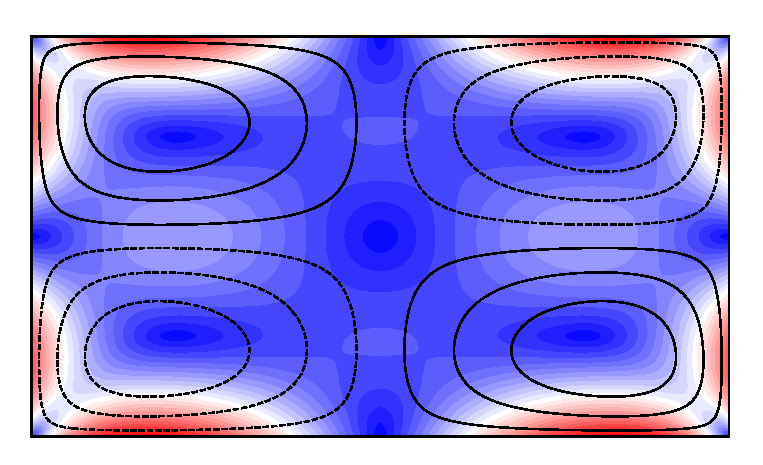
\includegraphics[width=0.45\textwidth] {figures/C4_streamline_1-1.eps}};
			\node (c12) at (4.25,0) {
				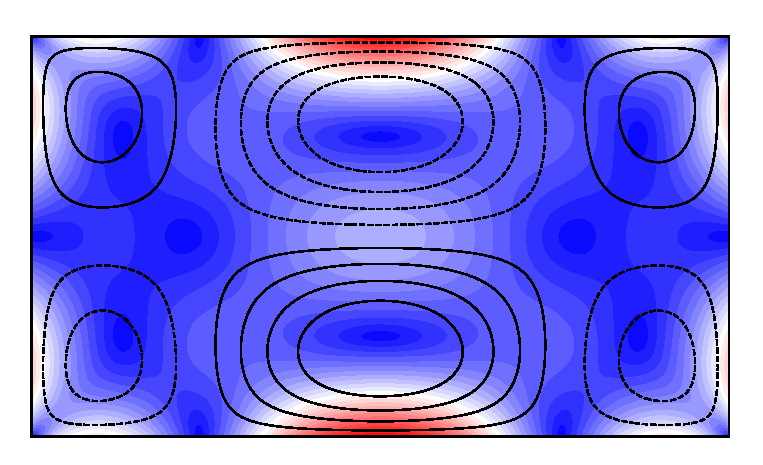
\includegraphics[width=0.45\textwidth] {figures/C4_streamline_2-1.eps}};
			\node (case) [above of=c11, xshift=-3.4cm, yshift=1.5cm] {B.C 4:};
			\node (a) [below of=case, xshift=-0.7cm, yshift=4mm] {(g)};
			\node (b) [right of=a, xshift=7.47cm] {(h)};
			
			\node [below of=c11, yshift=-1.5cm] {$x$};
			\node [left of=c11, xshift=-3cm] {$y$};
			
			\node [below of=c12, yshift=-1.5cm] {$x$};
			\node [left of=c12, xshift=-3cm] {$y$};
		\end{scope}
		\label{fig:eddy_gh}
		\begin{scope}[xshift=-7cm, yshift=-18.4cm]
			\pgfplotscolorbardrawstandalone[ 
			colorbar horizontal,
			colormap={mybwr}{samples of colormap=(25 of bwr)},
			colormap access=piecewise constant,
			point meta min=0,
			point meta max=1,
			colorbar style={
				width=14cm,
				height=2.5mm,
				xtick={0,0.2,0.4,...,1}
				}]
			\node at (7.1,-1.1) 
			{$\left| J_{xy}\right| / 
				\left| J_{xy}\right|_{\rm max}$};
		\end{scope}
	\end{tikzpicture}
	\caption{The induced current streamlines superposed over the normalized current density distribution at a horizontal $x$-$y$ plane located at $z = -h/2$. Sub-figures a), c), e) and g) pertain to the wave mode $(1,1)$ and b), d), f) and h) pertain to the wave mode $(2,1)$. Solid and dashed lines distinguish opposite current paths.}
	\label{fig:eddy_currents}
\end{figure}
%%%%%%%%%%%%%

%%%%%%%%%%%%%
\begin{figure}
	\begin{tikzpicture}
		\begin{scope}
			\node (c11) at (-4.25,0) {
				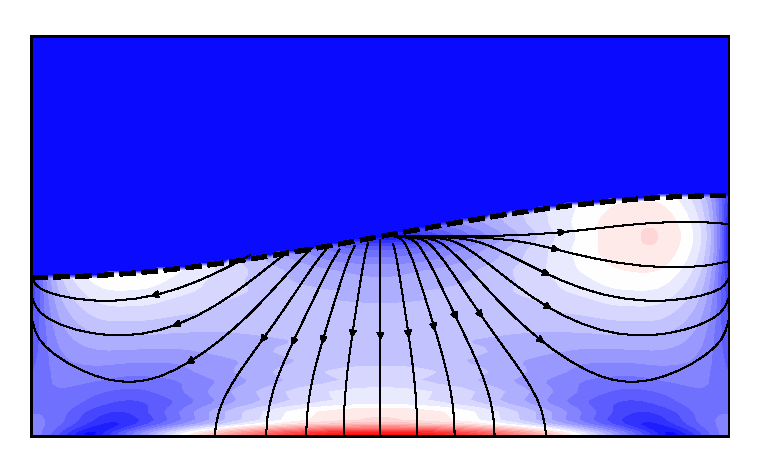
\includegraphics[width=0.45\textwidth] {figures/C3_XZ_1-1.eps}};
			\node (c12) at (4.25,0) {
				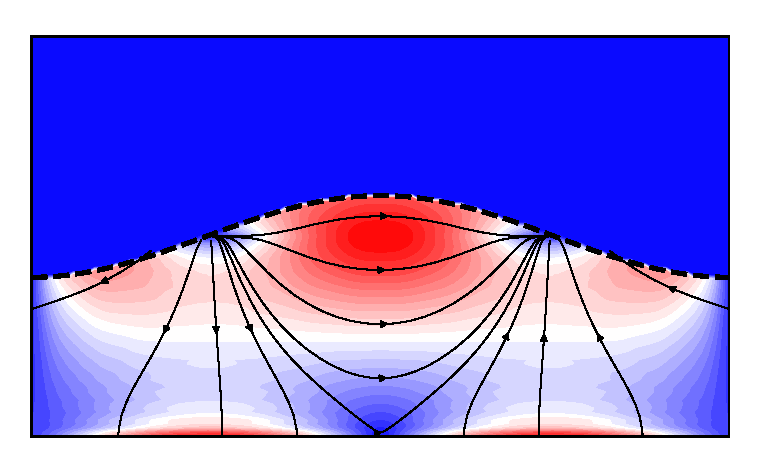
\includegraphics[width=0.45\textwidth] {figures/C3_XZ_2-1.eps}};
			\node (case) [above of=c11, xshift=-3.4cm, yshift=1.5cm] {B.C 3:};
			\node (a) [below of=case, xshift=-0.7cm, yshift=4mm] {(a)};
			\node (b) [right of=a, xshift=7.47cm] {(b)};
			
			\node [below of=c11, yshift=-1.5cm] {$x$};
			\node [left of=c11, xshift=-3cm] {$z$};
			
			\node [below of=c12, yshift=-1.5cm] {$x$};
			\node [left of=c12, xshift=-3cm] {$z$};
		\end{scope}
		\begin{scope}[yshift=-5.3cm]
			\node (c11) at (-4.25,0) {
				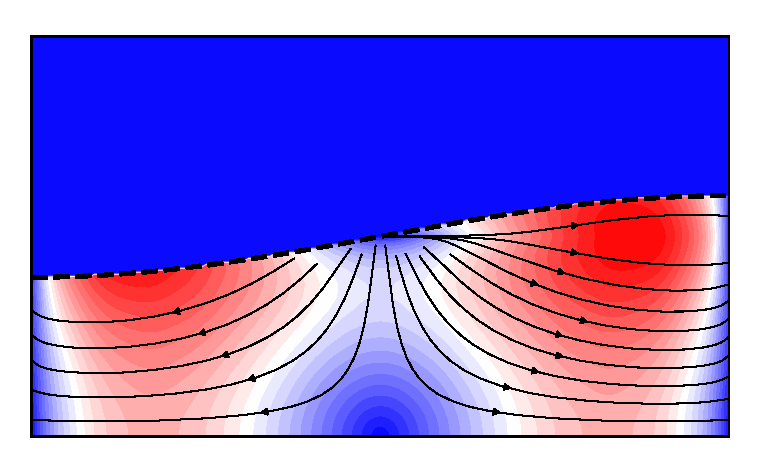
\includegraphics[width=0.45\textwidth] {figures/C4_XZ_1-1.eps}};
			\node (c12) at (4.25,0) {
				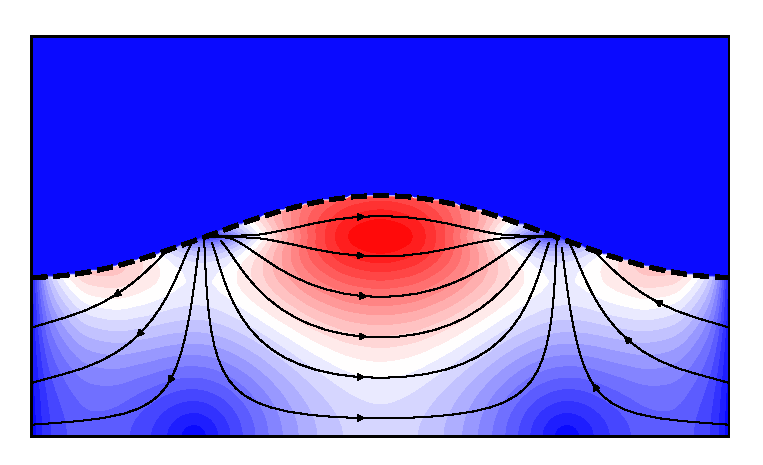
\includegraphics[width=0.45\textwidth] {figures/C4_XZ_2-1.eps}};
			\node (case) [above of=c11, xshift=-3.4cm, yshift=1.5cm] {B.C 4:};
			\node (a) [below of=case, xshift=-0.7cm, yshift=4mm] {(c)};
			\node (b) [right of=a, xshift=7.47cm] {(d)};
			
			\node [below of=c11, yshift=-1.5cm] {$x$};
			\node [left of=c11, xshift=-3cm] {$z$};
			
			\node [below of=c12, yshift=-1.5cm] {$x$};
			\node [left of=c12, xshift=-3cm] {$z$};
		\end{scope}
		
		\begin{scope}[xshift=-7cm, yshift=-7.8cm]
			\pgfplotscolorbardrawstandalone[ 
			colorbar horizontal,
			colormap={mybwr}{samples of colormap=(25 of bwr)},
			colormap access=piecewise constant,
			point meta min=0,
			point meta max=1,
			colorbar style={
				width=14cm,
				height=2.5mm,
				xtick={0,0.2,0.4,...,1}
			}]
			\node at (7.1,-1.1) 
			{$\left|J_{xz}\right| / 
				\left|J_{xz}\right|_{\rm max}$};
		\end{scope}
	\end{tikzpicture}
	\caption{The normalized induced current density superposed on the streamlines at a cross-section $y=L_y/2$ in the $x$-$z$ plane. Sub-figures a) and b) show this for wave modes $(1,1)$ and $(2,1)$, respectively, for B.C 3; sub-figures c) and d) show the same for B.C 4.}
	\label{fig:eddy_XZ}
\end{figure}
%%%%%%%%%%%%%


%%%%%%%%%%%%%%%%
\begin{figure}
\begin{tikzpicture}
	\node (pic1) [draw, black, inner sep=1pt] at (-5,0) 
	{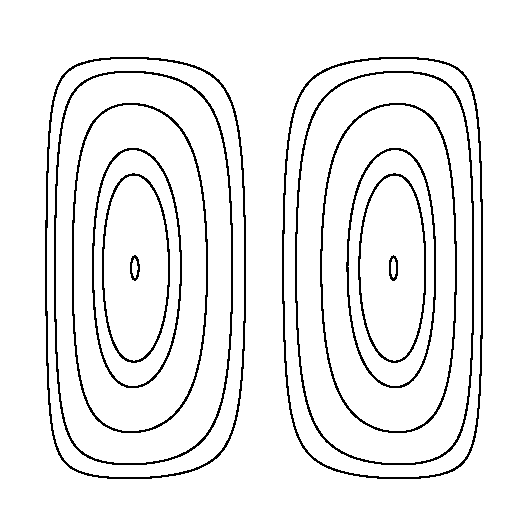
\includegraphics[width=0.2\textwidth]{figures/10.eps}};
	\node (pic2) [draw, black, inner sep=1pt, right of=pic1, xshift=3.3cm]
	{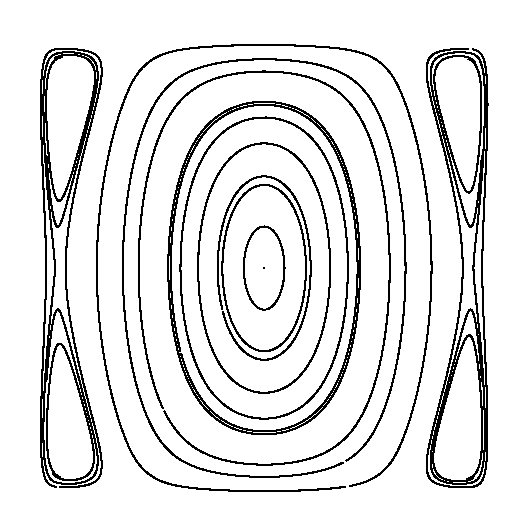
\includegraphics[width=0.2\textwidth]{figures/20.eps}};
	\node (pic3) [draw, black, inner sep=1pt, right of=pic2, xshift=3.3cm]
	{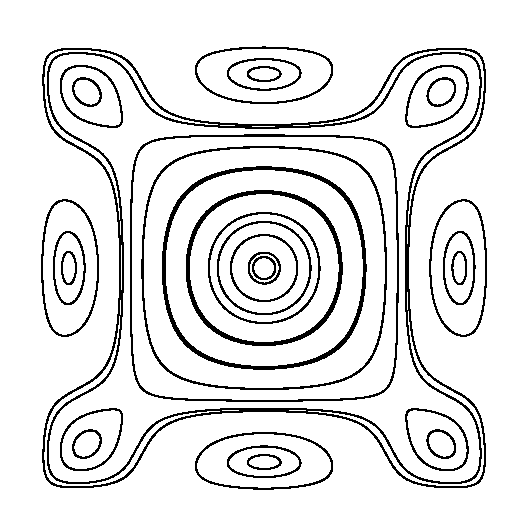
\includegraphics[width=0.2\textwidth]{figures/22.eps}};
	\node (pic4) [draw, black, inner sep=1pt, right of=pic3, xshift=3.3cm]
	{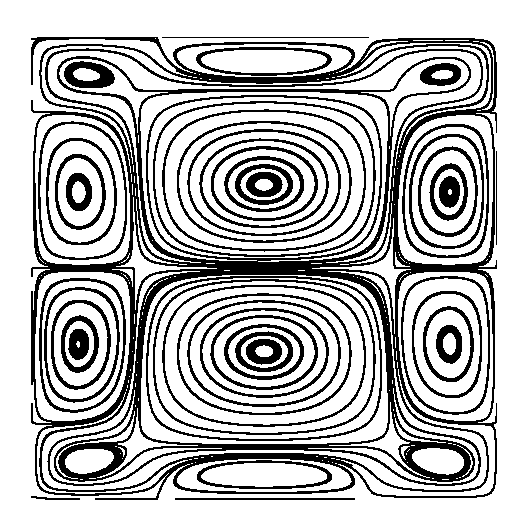
\includegraphics[width=0.2\textwidth]{figures/23.eps}};
	
	\node [left of=pic1,xshift=-1cm] {$y$};
	\node [below of=pic1,yshift=-1cm] {$x$};
	\node [left of=pic2,xshift=-1cm] {$y$};
	\node [below of=pic2,yshift=-1cm] {$x$};
	\node [left of=pic3,xshift=-1cm] {$y$};
	\node [below of=pic3,yshift=-1cm] {$x$};
	\node [left of=pic4,xshift=-1cm] {$y$};
	\node [below of=pic4,yshift=-1cm] {$x$};	
	
	\node [above of=pic1, xshift=-1.15cm, yshift=1.15cm] {(a) $(1,0)$};
	\node [above of=pic2, xshift=-1.15cm, yshift=1.15cm] {(b) $(2,0)$};
	\node [above of=pic3, xshift=-1.15cm, yshift=1.15cm] {(c) $(2,2)$};
	\node [above of=pic4, xshift=-1.15cm, yshift=1.15cm] {(d) $(2,3)$};
\end{tikzpicture}
\caption{ More examples of induced eddy current streamlines in the horizontal $x$-$y$ plane for wave modes a) $(1,0)$, b) $(2,0)$, c) $(2,2)$ and d) $(2,3)$. The total number of induced eddy currents for a given wave mode $(m,n)$ is observed to be equal to $(m+1)(n+1)$.}
\label{fig:eddy_examples}
\end{figure}

Since the expanded solutions of the electric potentials are very intricate and the eddy current patterns induced by the wave motions have not yet been analyzed for non-zero wave modes, we want to dive deeper into the underlying physics and examine the solution of the induced current density graphically. For this purpose, we consider a pair of non-zero wave modes $(1,1)$ and $(2,1)$ as shown in Fig.\,\ref{fig:wave_modes} and plot the induced current density distribution and streamlines formed at a horizontal plane (outlined in red in Fig.\,\ref{fig:wave_modes}) with vertical co-ordinates $z=-h/2$. This is shown in Fig.\,\ref{fig:eddy_currents} for all the four boundary conditions. The streamlines have been superimposed on the normalized planar current density distribution using the local maximum. The horizontal induced current densities are given by:
\begin{equation}
	\begin{bmatrix}
		J_x
		\\[5pt]
		J_y
	\end{bmatrix}
	=
	-\sigma
	\begin{bmatrix}
		\partial_x\Psi
		\\[5pt]
		\partial_y\Psi
	\end{bmatrix}
	+
	\sigma
	\begin{bmatrix}
		\partial_y\phi \,B_z
		\\[5pt]
		-\partial_x\phi\, B_z
	\end{bmatrix}
	\label{eq:eddy_current_vector}
\end{equation}  
Figs.\,\ref{fig:eddy_currents}\hyperref[fig:eddy_ab]{(a)} and \ref{fig:eddy_currents}\hyperref[fig:eddy_ab]{(b)} show the eddy current distribution for waves modes $(1,1)$ and $(2,1)$, bounded by perfect conductors as sidewalls (B.C 1) respectively. The solid and dashed lines represent opposite direction of eddy current flow. The pure horizontal currents $\h J=\sigma({\h u}\times B_z\h e_z)$, have no boundary corrections and and therefore, recirculate in the wall. When all sidewalls are conducting, the distribution of current density remain the same, regardless of the electrical boundary condition of the bottom wall. In B.C 2, the streamlines close only in the two conducting walls perpendicular to the $x$-axis, as shown in Figs.\,\ref{fig:eddy_currents}\hyperref[fig:eddy_ef]{(c)} and \ref{fig:eddy_currents}\hyperref[fig:eddy_ef]{(d)}. Figs.\,\ref{fig:eddy_currents}\hyperref[fig:eddy_cd]{(e)} and \ref{fig:eddy_currents}\hyperref[fig:eddy_cd]{(f)} refer to the eddy current distribution for the B.C 3 boundary configuration and Figs.\,\ref{fig:eddy_currents}\hyperref[fig:eddy_gh]{(g)} and \ref{fig:eddy_currents}\hyperref[fig:eddy_gh]{(h)} show the same for B.C 4. In both cases, we observe similar eddy current streamlines, but different current density distributions. In B.C 3, the induced currents cannot leave through the sidewalls due to the insulating boundary condition but close through the bottom wall. This can be seen in Figs.\,\subref{fig:eddy_XZ}{a} and \subref{fig:eddy_XZ}{b}, which shows the current distribution and current streamlines at a vertical cross-section at $y=L_y/2$ for wave modes $(1,1)$ and $(2,1)$ respectively. Here, we observe a greater concentration of currents at the bottom wall $z=-h$. Figs.\,\subref{fig:eddy_XZ}{c} and \subref{fig:eddy_XZ}{d} show the current distribution at $y=L_y/2$ in the $x$-$z$ plane for B.C 4 respectively, which is characterized by stronger current densities near the free surface and the redirection of the currents near the insulating bottom wall. It is evident that B.C 3 has higher magnitudes of $J_z$ compared to B.C 4 and, naturally, B.C 2. The difference in current distribution between cases B.C. 3 and B.C. 4, which have the same sidewall boundary conditions except for the bottom wall, is a key result to note when discussing the magnetic damping rate in Sec.\,\ref{sec:mag_damp}. 
\\
\indent By analyzing the solutions in detail, we can deduce an observed rule for the total number of all the eddies that are formed $n_{\rm eddy}$, as a function of the wave mode indices:
\begin{equation}
	n_{\rm eddy} = (m+1)\,(n+1).
	\label{eq:no_of_eddies}
\end{equation}     
Further examples of eddy current streamlines are given in Fig.\,\ref{fig:eddy_examples} for both uni- and bidirectional wave modes pertaining to the B.C 4 case. Wave modes $(1,0)$, $(2,0)$, $(2,2)$ and $(2,3)$ give rise to 2, 3, 9 and 12 distinct eddies in the horizontal plane respectively. It is evident that the wave modes as well as the boundary conditions clearly have an influence in the complex behavior of the eddy patterns, both in their spatial arrangement and the size distribution. 
 
\subsection{Ohmic dissipation}
\label{sec:ohmic_dissipation}

\indent Having obtained the solutions of $\Psi$ in terms of a series harmonic and hyperbolic functions, we can now solve for $\h J$ and therefore the damping rate due to Ohmic dissipation, which we denote by $\lambda_{\rm o}$. Neglecting the viscosity and surface tension, the mechanical energy balance reads
\begin{equation}
	 \dv{}{t}\left( \frac{1}{2} 
	 \int_{V} \rho \norm{\h u}^2 \mathrm dV  \right)
	 +
	 \dv{}{t}\left( \int_{\mathcal{S}} 
	 \frac{1}{2} \rho \:g\eta^2  \: \mathrm d\mathcal{S}  
	 \right)
	  = -
	  \int_{V} \frac{1}{\sigma} \h J^2 \: \mathrm dV ,
	  \label{eq:balance_ohmic}
\end{equation}
which states that the sum of the rate of kinetic energy in the bulk and the potential energy in the free surface is equal to the total energy dissipated. The detailed analytical calculation is provided in Sec.\,\RN{2} of the supplementary material \cite{SMmagdamp_hegde}. The expression for $\lambda_{\rm o}$ obtained after accounting for the mean Ohmic loss over a wave cycle, is as follows:
\begin{equation}
	\lambda_{\rm o} = 
	\dfrac{
		\mathcal{Q}_{\rm ind}
		-\mathcal{Q}_{\rm corr}	}{2 K},
	\label{eq:mag_damping_rate_short}
\end{equation}
where $\mathcal{Q}_{\rm ind}$ is the dissipation of energy due to induced currents. The expression for $\mathcal{Q}_{\rm ind}$ for all cases are:
\begin{equation}
	\mathcal{Q}_{\rm ind} = 
	\sigma \int_{V}  \norm{\bm{\nabla} {\phi}\times B_z\bm e_z}^2
	=
	A^2_{mn}
	\epsilon_{m}\epsilon_{n}\frac{ \sigma
		\omega^2B_z^2(\coth[kh]+kh\csch^2{[kh]})}{8k}L_xL_y ,
		\quad 
	\epsilon_{r} =
	\biggl\{ \begin{array}{rc}
		2,  & r= 0 \\
		1,  & r\neq 0
	\end{array}	,
	\label{eq:qind}
\end{equation}
and $\mathcal{Q}_{\rm corr}$ is the correction to the dissipation due to insulating/conducting wall boundary conditions, given by the integral
\begin{equation}
	\mathcal{Q}_{\rm corr} =
	\int_{V} \bm{\nabla} {\phi}\cdot (-\sigma \bm{\nabla}{\Psi} \times B_z\bm{e}_z ),
	\label{eq:Qcorr_integral}
\end{equation}
which varies depending on the electric potential $\Psi$. The term $K$ is proportional to the kinetic/potential energy of the standing wave ($m,n$). It is given by
\begin{equation}
	K = 0.25 A^2_{mn}\epsilon_{m}\epsilon_{n} \rho g L_xL_y.
	\label{eq:K_eq}
\end{equation}
The correction term $\mathcal{Q}_{\rm corr}$ mainly originates from insulating sidewalls. In a domain with both insulating and conducting sidewalls, the correction terms from each pair of insulating walls are subtracted from the dissipation term if all walls were conducting. In B.C 1, or in a domain with all four sidewalls as perfect conductors, the correction term ${\mathcal{Q}}_{\rm corr} = 0$, as the current densities close in the walls $\bigl($see Fig.\,\ref{fig:eddy_currents}\hyperref[fig:eddy_ab]{(a)} and  \ref{fig:eddy_currents}\hyperref[fig:eddy_ab]{(b)}$\bigr)$. 
\\
\indent In B.C 2, involving one pair of insulating sidewalls, results in:
\begin{equation}
	{\mathcal{Q}}_{\rm corr} (\ii{B.C 2}) = 
	A_{mn}  \left[
	\sum_{b=0}^{\infty} 
	\frac{
		-\grave{\mathcal B}_{mb} \; \sigma\omega B_z \:
		 m\pi (-1)^{n+b} 	}
	{
		\left(
		\dfrac{1-(-1)^n}{2\cosh{\bigl[0.5\grave\xi_y L_y]}} + \dfrac{1+(-1)^n}{2\sinh{\bigl[0.5\grave\xi_y L_y]}}
		\right)
	}
	\frac{h^2}{(k^2h^2 +  b^2\pi^2)}
	\right] ,
	\label{eq:qcorr_bc2}
\end{equation}
as the pair of conducting walls parallel to the $y$-axis do not contribute to the correction term; which is why $\grave{\mathcal{Q}}_{\rm corr} = 0$ for a unidirectional wave along the $y$-axis ($m=0,\,y\neq0$). The terms $\grave{\mathcal B}_{mb}$ and $\grave\xi_y$ are given in Eq.\,\eqref{eq:bc2_B}.
\\
\indent The correction term for B.C 3 is
\begin{align}
	\nn
	&\mathcal{Q}_{\rm corr}  (\ii{B.C 3})= 
	A_{mn} \left[ \rule{0pt}{0.9cm} 
	\tilde{\mathcal A}_0 \sigma\omega B_z 
	\left( \dfrac{ \tilde\Delta_{m,n}\tanh{[0.5p_hL_x]}
	+
	\tilde{\tilde{\Delta}}_{m,n}\coth{[0.5p_hL_x]}
	}
	{2\pi(m^2h^2+0.25L_x^2)} \right)
	\dfrac{h^2L_x^2(\pi\csch{[kh]} + 2kh)}
	{k(4k^2h^2+\pi^2)}
	\right.
	\\
	\nn
	&- 
	\tilde{\mathcal B}_0 \sigma\omega B_z 
	\left( \dfrac{ \tilde\Delta_{n,m}\tanh{[0.5p_hL_y]}
		+
		\tilde{\tilde{\Delta}}_{n,m}\coth{[0.5p_hL_y]}
	}
	{2\pi(n^2h^2+0.25L_y^2)} \right)
	\dfrac{h^2L_y^2(\pi\csch{[kh]} + 2kh)}
	{k(4k^2h^2+\pi^2)}
	\\
	\nn
	&+ 
	\sum_{\substack{a, b \geq 0 \\ (a,b) 
			\neq (0,0) \\
			a\neq n	
	}}^{\infty}
		\frac{ 
		4 \tilde{\mathcal A}_{ab} \,\omega\sigma B_z \:
		(a^2m^2\pi^2 + {\tilde\xi_x}^2n^2L_x^2)
		\Bigl( (-1)^{m+1} + (-1)^{a+m+n} \Bigr) }
	{(a^2-n^2) (m^2\pi^2 + {\tilde\xi_x}^2L_x^2)
		\left(
		\dfrac{1-(-1)^m}{2\cosh{\bigl[0.5\tilde\xi_x L_x \bigr]}} + \dfrac{1+(-1)^m}{2\sinh{\bigl[0.5\tilde\xi_x L_x \bigr]}}
		\right)
	}\!
	\frac{h\Bigl( (1+2b)\pi\csch{[kh]} + 2kh(-1)^b \Bigr)}
	{k \Bigl( 4k^2h^2 + (1+2b)^2\pi^2 \Bigr)}
	\\
	&- \left.
	\sum_{\substack{a, b \geq 0 \\ (a,b) 
			\neq (0,0) \\
			a\neq m	
	}}^{\infty}
		\frac{ 4 \tilde{\mathcal B}_{ab} \,\omega\sigma B_z \:
		(a^2n^2\pi^2 + {\tilde\xi_y}^2m^2L_y^2)
		\Bigl( (-1)^{n+1} + (-1)^{a+m+n} \Bigr) }
	{(a^2-m^2) (n^2\pi^2 + {\tilde\xi_y}^2L_y^2)
		\left(
		\dfrac{1-(-1)^n}{2\cosh{\bigl[0.5\tilde\xi_y L_y]}} + \dfrac{1+(-1)^n}{2\sinh{\bigl[0.5\tilde\xi_y L_y]}}
		\right)
	}\!
	\frac{h\Bigl( (1+2b)\pi\csch{[kh]} + 2kh(-1)^b \Bigr)}
	{k \Bigl( 4k^2h^2 + (1+2b)^2\pi^2 \Bigr)}
	\rule{0pt}{1cm} \right],
	\label{eq:qcorr_bc3}
\end{align}
where,
\begin{equation}
	\tilde\Delta_{q,r} = (1+(-1)^q)(1-(-1)^r)^2,
	\qquad
	\tilde{\tilde{\Delta}}_{q,r} = (-1+(-1)^q)(1-(-1)^r)^2 .
\end{equation}
The constants $\tilde\xi_x$ and $\tilde\xi_y$ are given in Eq.\,\eqref{eq:bc3_xi}; and the coefficients $\tilde{\mathcal A}_0$, $\tilde{\mathcal B}_0$, $\tilde{\mathcal A}_{ab}$ and $\tilde{\mathcal B}_{ab}$ are given in Eqs.\,(\ref{eq:bc3_constantsA0}, \ref{eq:bc3_constantsB0}, \ref{eq:bc3_A} and \ref{eq:bc3_B}) respectively. 
\\
\indent Similarly, in B.C 4, the correction term takes the following form:
\begin{align}
	\nn
	\mathcal{Q}_{\rm corr}  (\ii{B.C 4}) &=
	A_{mn}  \left[ \rule{0pt}{1cm}
	- \ddot{\mathcal A}_0 \sigma\omega B_z L_x
	\dfrac{ \bigl( -1 + (-1)^n \bigr) }{k^2}\; \ddot\Delta_{m}
	+
	\ddot{\mathcal B}_0 \sigma\omega B_z L_y
	\dfrac{ \bigl( -1 + (-1)^m \bigr) }{k^2}\; \ddot\Delta_{n}
	\right.
	\\
	\nn
	& +
	\sum_{\substack{a, b \geq 0 \\ (a,b) 
			\neq (0,0) \\
			a\neq n	
	}}^{\infty}
	\frac{ 2 \ddot{\mathcal A}_{ab} \sigma \omega B_z 
		\:(a^2m^2\pi^2 + {\ddot\xi_x}^2n^2L_x^2)
		\Bigl( (-1)^{b+m+1} + (-1)^{a+b+m+n} \Bigr) }
	{(a^2-n^2) (m^2\pi^2 + {\ddot\xi_x}^2L_x^2)
		\left(
		\dfrac{1-(-1)^m}{2\cosh{\bigl[0.5\ddot\xi_x L_x \bigr]}} + \dfrac{1+(-1)^m}{2\sinh{\bigl[0.5\ddot\xi_x L_x \bigr]}}
		\right)
	}
	\frac{h^2}{(k^2h^2 + b^2\pi^2)}
	\\
	& - 
	\left.
	\sum_{\substack{a, b \geq 0 \\ (a,b) 
			\neq (0,0)\\
			a\neq m	
	}}^{\infty}
	\frac{ 	2 \ddot{\mathcal B}_{ab} \sigma \omega B_z 
		\: (a^2n^2\pi^2 + {\ddot\xi_y}^2m^2L_y^2)
		\Bigl( (-1)^{b+n+1} + (-1)^{a+b+m+n} \Bigr) }
	{(a^2 - m^2)
		(n^2\pi^2 + {\ddot\xi_y}^2L_y^2)
		\left(
		\dfrac{1-(-1)^n}{2\cosh{\bigl[0.5\ddot\xi_y L_y \bigr]}} + \dfrac{1+(-1)^n}{2\sinh{\bigl[0.5\ddot\xi_y L_y \bigr]}}
		\right)
	}
		\frac{h^2}{(k^2h^2 + b^2\pi^2)}
	\rule{0pt}{1cm} \right] ,
	\label{eq:qcorr_bc4}
\end{align} 
where, 
\begin{equation}
	\ddot\Delta_{m}=
	\left\{
	\begin{array}{rl}
		1, & m=0, n\neq 0 \\
		\dfrac{(-1)^n \bigl(1 - (-1)^m \bigr)^2}{m^2\pi^2}, & m, n\neq 0
	\end{array}
	\right.
	,\quad
	\ddot\Delta_{n}=
	\left\{
	\begin{array}{rl}
		1, & n=0, m\neq 0 \\
		\dfrac{(-1)^m \bigl(1 - (-1)^n \bigr)^2}{n^2\pi^2}, & m, n\neq 0
	\end{array}
	\right. .
	\label{eq:qcorr_bc3_consts}
\end{equation}
In Eq.\,\eqref{eq:qcorr_bc4}, the coefficients $\ddot{\mathcal A}_0$, $\ddot{\mathcal B}_0$ are given in Eq.\,\eqref{eq:bc4_constants}, and $\ddot{\mathcal{A}}_{ab}$ and $\ddot{\mathcal B}_{ab}$ are given in Eqs.\,(\ref{eq:bc4_Acoeff} and \ref{eq:bc4_Bcoeff}) respectively.   
\\
\indent All of the correction terms from Eqs.\,(\ref{eq:qcorr_bc2}, \ref{eq:qcorr_bc3} and \ref{eq:qcorr_bc4}) are quite cumbersome to translate into code or analytical solvers. Therefore, we have outlined all of the formulae in a Python script to make it easier for readers to perform the calculations.  


\subsection{Hartmann and Shercliff boundary layers}
\label{sec:hartmann_and_shercliff}

In addition to Ohmic dissipation in the bulk, the effect of the magnetic field on the boundaries must be taken into consideration. In an electrically conducting fluid system, the presence of a magnetic field alters the standard hydrodynamic boundary layers depending on the field intensity. The velocity profile at the walls have two distinct layers, called the Hartmann and Shercliff layers. Hartmann boundary layers are formed at surfaces perpendicular to the direction of the applied magnetic field, whereas Shercliff layers are formed parallel to them. It is well known that the thickness of the Hartmann layers scale inversely with Ha $(\delta_{\rm Ha} \sim \textrm{Ha}^{-1})$ \cite{Hartmann, shercliff1981, Muller2001}. This implies that increasing the magnetic field strength reduces the overall thickness while increasing overall dissipation at the wall. Shercliff layers, unlike Hartmann layers do not directly contribute in braking the fluid velocity but redistribute the induced currents and fluid momentum throughout the system. They are usually thicker than the Hartmann layers as they scale inversely to the square root of $\rm Ha$ $(\delta_{\rm Sh} \sim \textrm{Ha}^{-0.5})$ \cite{shercliff1981}. 
\\
\indent In our setup, the Hartmann layer forms only at the bottom wall of the domain. The Shercliff layers form at the four sidewalls of the rectangular domain, which are parallel to the applied magnetic field. In principle, these layers are the result of the Stokes boundary layer transitioning under the influence of the magnetic field. They are a combination of the conventional Hartmann or Shercliff layers with the respective oscillating Stokes boundary layer \cite{Sreenivasan2005}. Therefore we can follow the methodology of \citet{Keulegan1959} in resolving the Stokes boundary layers for free surface waves in a rectangular domain. We can then incorporate the effects of Lorentz forces due to induced currents \cite{Davidson2001}. The inviscid formulation of the velocity $\h u=\bm\nabla\phi$ already satisfies the condition of impermeability at the boundary. However, in order to model the tangential velocity and stress at the boundary, we need to enforce the following corrections to the potential wave solutions of velocity and pressure:
\begin{subequations}
\begin{align}
	\h u &= \left[\bm\nabla\phi
	 + {\overbar{\h u}}\:  \ii e^{ \ii{i}\omega t} \right]\ii e^{-\lambda_{\ii b}t},
	 \label{eq:velocity_correction}
	\\
	p &=  \left[ -\rho(\ii i\omega)\phi
	+ {\overbar{p}}\:  \ii e^{ \ii{i}\omega t}
	\right]\ii e^{-\lambda_{\ii b}t},
	\label{eq:pressure_correction}
\end{align}
\end{subequations}
with ${\overbar{\h u}}$ and ${\overbar{p}}$ as the corrections to the potential flow velocity and pressure respectively. The term $\lambda_{\rm b}$ in the exponent is the damping rate of the standing wave solely due to boundary layer effects. Considering only the tangential velocities ${\bar{\h u}}_{\perp}$ at the respective boundaries and the damping force by virtue of induction, the linearized Navier-Stokes momentum equation [Eq.\,\eqref{eq:gov_momentum}] reduces to
\begin{equation}
	\ii{i}\omega {\bar{\h u}}_{\perp} = -\frac{1}{\rho}\bm\nabla_{\perp}{\overbar{p}} 
	+ \nu\pdv[2]{{\overbar{\h u}}_{\perp}}{\zeta}
	- \frac{\sigma B_z^2}{\rho} {{\h u}}_{b} ,
	\label{eq:gov_stokes_general}
\end{equation}
in the leading order. In Eq.\,\eqref{eq:gov_stokes_general}, $\zeta$ is the spatial coordinate normal to the wall that reduces the boundary layer corrections to zero away from the wall:
\begin{equation}
	\zeta = \begin{cases}
		z + h, \quad &\text{near } z=-h, \\
		\dfrac{L_x}{2} - x, \quad &\text{near } x = L_x/2, \qquad\qquad
		x + \dfrac{L_x}{2}, \quad \text{near } x = -L_x/2 \\[5pt]
		\dfrac{L_y}{2} - y, \quad &\text{near } y = L_y/2, \qquad\qquad
		y + \dfrac{L_y}{2}, \quad \text{near } y = -L_y/2,
	\end{cases} ,
\end{equation}
and ${{\h u}}_{b}$ is the velocity in the boundary layer. In the leading order, the normal part of the mass and momentum balance is zero i.e. $\partial_\zeta {\bar{\h u}} \cdot \h n = 0$ and ${\bar{p}} = 0$ respectively. The tangential velocities decay exponentially away from the boundary, ${\bar{\h u}}_{\perp} \sim \ii e^{-\zeta/\delta_{\rm tot}}$, where $\delta_{\rm tot}$ is the total thickness of the boundary layer. The inverse of $\delta_{\rm tot}$ signifies the sharpness of the velocity gradient near the boundary. In context to the Hartmann layer, the velocity at the boundary scales as ${{\h u}}_{b} \sim {\bar{\h u}}_{\perp}$. We can therefore solve for $\delta_{\rm tot}$ in Eq.\,\eqref{eq:gov_stokes_general} to obtain
\begin{equation}
	\delta_{\rm tot} (\ii{Ha}) =
	\left[
	\ii{Re}\sqrt{\dfrac{\ii i\omega}{\nu} + \dfrac{1}{\tau\nu} }
	\:\right]^{-1}
	=\frac{\sqrt{2\tau\nu}}{\sqrt{1+\sqrt{1+\tau^2\omega^2}}}
	= 
	\left( \frac{1}{2} \Bigl(
	\delta_{\rm Ha}^{-2} + \left( \delta_{\rm Ha}^{-4} + 4\delta_{\rm v}^{-4}\right)^{0.5} \Bigr)
	\right)^{-0.5}
	,
	\label{eq:hartmann_layer_thickness}
\end{equation}
which is the total boundary layer thickness at the wall normal to the magnetic field. Here $\tau$ is denoted as the characteristic damping time given by
\begin{equation}
	\tau  = \frac{\rho}{\sigma B_z^2} .
	\label{eq:damping_time}
\end{equation}
The boundary layer Eq.\,\eqref{eq:hartmann_layer_thickness} is composed of both the Stokes ($\delta_{\rm v} = \sqrt{2\nu/\omega}$) and the Hartmann boundary ($\delta_{\rm Ha}=\sqrt{\tau\nu}$) layers. However, there is no straight forward equation that can be used to calculate the expression for the Shercliff boundary layer. But we can approximate the total thickness using the conservation of currents. In a given fluid layer, the currents close as they pass through the horizontal Hartmann layers of thickness $\delta_{\rm Ha}$ and the vertical Shercliff layers over the entire fluid depth $h$. Therefore, we write the following relation:
\begin{equation}
	\sigma{\overbar{u}}_{\perp} B_z \delta_{\rm Ha} \sim 
	\sigma
	{u}_b B_z h 
	\Longrightarrow 
	{u}_b \sim \frac{\delta_{\rm Ha}}{h} 
	\;{\overbar{u}}_{\perp}.
	\label{eq:shercliff_relation}
\end{equation} 
In Eq.\,\eqref{eq:shercliff_relation}, the current density in the Hartmann layer scales with the current density in the Shercliff layer over the fluid height. Substituting Eq.\,\eqref{eq:shercliff_relation} in \eqref{eq:gov_stokes_general}, we get the total boundary layer thickness at the sidewalls parallel to the magnetic field:
\begin{equation}
	\delta_{\rm tot} (\ii{Sh}) \approx 
	\left[ \rule{0pt}{0.8cm}
	\ii{Re}\sqrt{\dfrac{\ii i\omega}{\nu} + \dfrac{1}{h\sqrt{\tau\nu}}
	}
	\:\right]^{-1}
	=
	\dfrac{\sqrt{2h\sqrt{\tau\nu}}}
	{
		\sqrt{1 + \sqrt{1 + \dfrac{\tau h^2\omega^2}{\nu}}}
	}
	= 
	\left( \frac{1}{2}\Bigl(
	\delta_{\rm Sh}^{-2} + \left( \delta_{\rm Sh}^{-4} + 4\delta_{\rm v}^{-4}\right)^{0.5} \Bigr)
	\right)^{-0.5}
	,
	\label{eq:shercliff_layer_thickness}
\end{equation}
where the conventional Shercliff layer scales with the square root of the Hartmann layer thickness, $\delta_{\rm Sh} \sim \sqrt{h\,\delta_{\rm Ha}}$. Therefore, the tangential velocity corrections in the Hartmann and Shercliff layers are
\begin{equation}
	{\overbar{\h u}}_{\perp} (\ii{Ha})=
	-\bm\nabla \phi 
	\ii e^{-
		\sqrt{\dfrac{\ii i\omega}{\nu} + \dfrac{1}{\tau\nu}
		}
	\zeta
	},
	\qquad
	{\overbar{\h u}}_{\perp} (\ii{Sh})=
	-\bm\nabla \phi 
	\ii e^{- 
		\sqrt{\dfrac{\ii i\omega}{\nu} + \dfrac{1}{h\sqrt{\tau\nu}}
		}
		\zeta
	},
	\label{eq:Ha_Sh_velocities}
\end{equation}
which contribute to the damping rates of a standing wave solely due to the dissipation of energy in the Hartmann-viscous layer and the Shercliff-viscous layer respectively. We denote the damping rates as $\lambda_{\ii{Ha}}$ and the $\lambda_{\ii{Sh}}$ respectively. 
%%%%%%%%%%%%%
\begin{table}%[H] add [H] placement to break table across pages
	\caption{Cell parameters and material properties from \citet{Bojarevics2006a}.}
	\label{tab:table_bojarevics_prop}
	\begin{ruledtabular}
		\begin{tabular}{llll}
			
			Length of cell ($L_x$): & \SI{0.154}{\meter}  &
			&
			\\
			Breadth of cell ($L_y$): 	& \SI{0.094}{\meter}  &
			&  
			\\[5pt]
			Properties of GaInSn ($\Omega$) &  &  & \\
			Density ($\rho$):
			& \SI{6363}{\kilogram\per\meter\tothe{3}} & Electrical conductivity ($\sigma$):
			& \SI{3.31e6}{\siemens\per\meter}
			\\
			Kinematic viscosity ($\nu$):
			& \SI{3.48e-7}{\meter\tothe{2}\per\second} & Layer depth ($h$): &
			\SI{0.049}{\meter}
		\end{tabular}
	\end{ruledtabular}
\end{table}
%%%%%%%%%%
\indent To illustrate more clearly the effect of the Hartmann and Shercliff layers on the Stokes velocity profile, we calculate the boundary layer velocities in a single-layer liquid metal system from \citet{Bojarevics2006a}. We consider a free surface wave motion of mode $(1,0)$. The system is threaded by a constant vertical DC magnetic field of magnitude $B_z$. The properties of the materials are provided in Table\,\ref{tab:table_bojarevics_prop}. The velocity profiles from the bottom boundary to the free surface at different Hartmann numbers are presented in Fig.\,\subref{fig:stokes_vel}{a}. The velocities are plotted along the line $x=L_x/4$ in the $x$-$z$ plane, with $\ii{Ha} = B_zL_x\sqrt{\sigma/(\rho\nu)}$. Here, the term $\h u^*_{T} = ({\h u}_{x} + {\overbar{\h u}}_{x})/{\h u}_{x}$ is the non-dimensionalized total to bulk velocity ratio.  In the absence of the magnetic field ($\rm Ha=0$), the boundary reverts to the classical Stokes boundary layer with thickness $\delta_{\rm tot} = \sqrt{2\nu/\omega}$, which is highlighted in blue. The boundary layer thickness at $\rm Ha = 3000$ (highlighted in red) is minuscule in comparison to the case when $\rm Ha = 0$, as $\delta_{\rm tot}$ varies inversely with $\rm Ha$. At $z=-h$, the velocity ratio follows the Stokes profile where the correction cancels out the free stream velocity at the boundary. This is followed by the characteristic 'velocity overshoot', where the local velocity exceeds the bulk velocity momentarily and then converges to the bulk velocity after. This is due to the no-slip constraint enforced at the wall, which does not cause the corrections to fade monotonically but act like a damped oscillator (emphasized by the presence of a cosine term in the velocity) that approaches equilibrium \cite{Schlichting2016}. As the Hartmann number increases, the overshoots die down and are replaced by sharper velocity gradients and the boundary layer shrinks to Eq.\,\eqref{eq:hartmann_layer_thickness}. 
%%%%%%%%%%%%
\begin{figure}
	\centering
	\hspace{-1.5cm}
	\begin{tikzpicture}
		\begin{scope}[name prefix=scope1, xshift=-1.5cm]
			\node (pic1) at (0,0) 
			{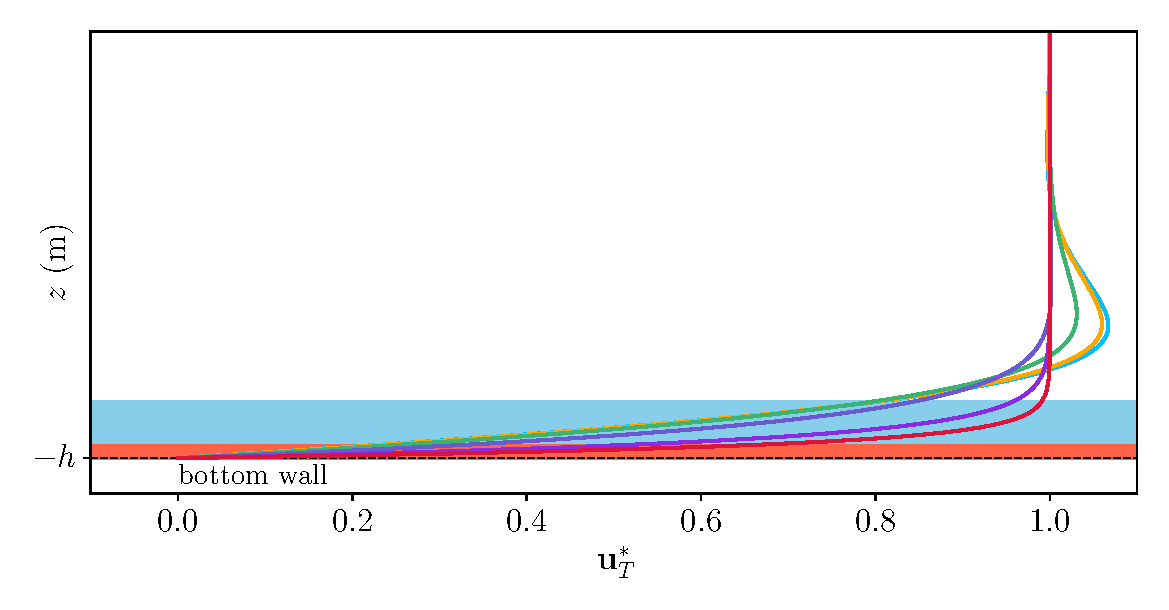
\includegraphics[height=6cm]{figures/stokes_vel_bottom.eps} };
			\node (a) [above left=-1cm of pic1] {(a)};
			
			\node (pic2) at (0,-6) 
			{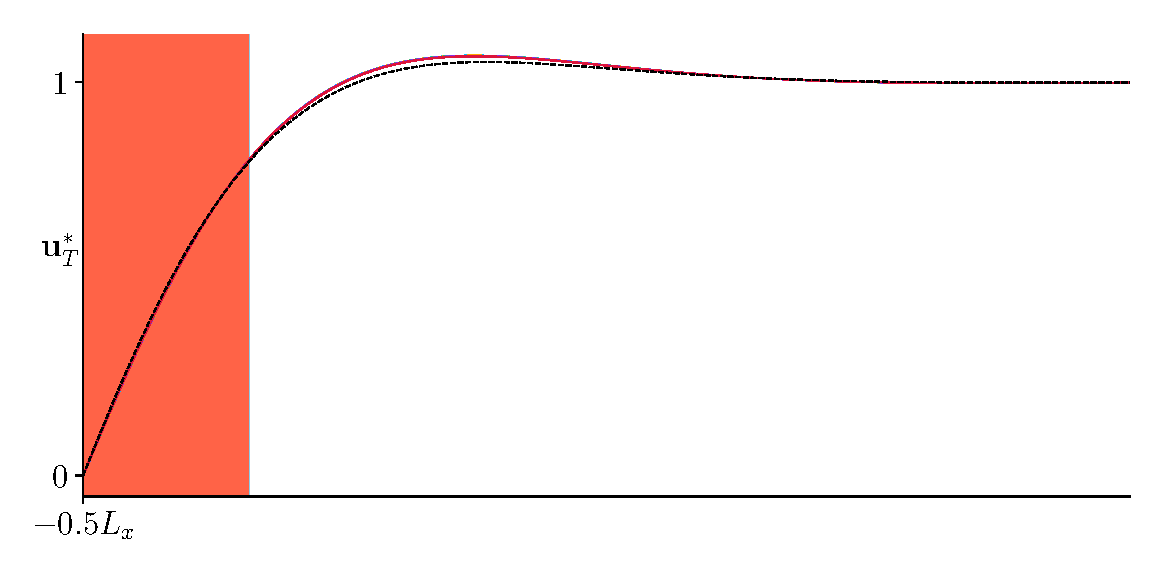
\includegraphics[height=5.54cm]{figures/stokes_vel_sher_zoom.eps} };
			\node (b) [below = 5.2cm of a] {(b)};
			\node [right = 0mm of b] {Near the wall:};
			\node [below = -0.65cm of pic2] {$x$ (m)};
			
			\draw (-2.5,-4) -- (-1.75,-4.5) node [right] {$\rm Ha = 30000$};
			
%			\draw [<->] (-4.8,-1.6)--(-4.8,-1) node [above] {$\delta_{\rm v}$};
%			\draw [<->] (-4.5,-1.6)--(-4.5,-1.45) node [above] {$\delta_{\rm tot}$};
%		% Grid
%		\draw[lightgray,step=0.5] (pic2.south west) grid (pic2.north east);
%		% Axes' labels
%		\foreach \x in {-6,-5,...,6} { \node [above] at (\x,-3) {\x}; }
%		\foreach \y in {-9,-8.5,...,-3} { \node [left] at (-6,\y) {\y};} 
			
		\end{scope}

		\begin{scope}[yshift=-9.1cm, xshift=-9cm]
			\coordinate (x1) at (0,0);
			\coordinate (x2) at (0.75,0);
			
			\draw [very thick, deepskyblue] (x1) -- (x2) node [right, black] {$\ii{Ha} = 0$};
			\draw [very thick, orange, transform canvas={xshift=2.3cm}] (x1) -- (x2) node [right, black] {$\ii{Ha} = 200$};
			\draw [very thick, mediumseagreen, transform canvas={xshift=4.8cm}] (x1) -- (x2) node [right, black] {$\ii{Ha} = 500$};
			\draw [very thick, slateblue, transform canvas={xshift=7.3cm}] (x1) -- (x2) node [right, black] {$\ii{Ha} = 1000$};
			\draw [very thick, blueviolet, transform canvas={xshift=10cm}] (x1) -- (x2) node [right, black] {$\ii{Ha} = 2000$};
			\draw [very thick, crimson, transform canvas={xshift=12.7cm}] (x1) -- (x2) node [right, black] {$\ii{Ha} = 3000$};
		\end{scope}

		\begin{scope}[yshift=-9.9cm, xshift=-4cm]
			\coordinate (r1) at (0,-0.1);
			\coordinate (r2) at (0.75,0.1);
			
			\path [fill=skyblue] (r1) rectangle (r2) node [right, black, yshift=-1.4mm] {$\delta_{\rm tot}$ ($\ii{Ha}=0$)};
			\path [fill=tomato, transform canvas={xshift=3.2cm}] (r1) rectangle (r2) node [right, black, yshift=-1.4mm] {$\delta_{\rm tot}$ ($\ii{Ha}=3000$)};
		\end{scope}
	\end{tikzpicture}
	\caption{The Stokes velocity profile in the $x$-$z$ plane for different $\rm Ha$ near the a) bottom wall along $x=L_x/4$, and b) near the sidewall ($-0.5L_x$) along $z=-h/2$. A quasi-2D unidirectional wave mode $(1,0)$ is considered.  The blue shaded region quantifies the viscous layer thickness whereas the red region shows the total boundary thickness including Hartmann and Shercliff layers in a) and b) respectively.}
	\label{fig:stokes_vel}
\end{figure}
%%%%%%%%%%%%
\\
\indent Fig.\,\subref{fig:stokes_vel}{b} shows the magnified view of velocity profile along the line $z=-h/2$ in the $x$-$z$ plane, near the sidewall at $x=-L_x/2$. When $\rm Ha = 3000$, we observe that the Shercliff layer is identical to the conventional viscous sub layer ($\rm Ha = 0$), and is significantly thicker than the Hartmann layer at the bottom. The velocity ratio is $\h u^*_{T}=({\h u}_{z} + {\overbar{\h u}}_{z})/{\h u}_{z}$ in this case. The Stokes overshoot profile remains noticeable for all cases of $\rm Ha$ considered; the magnetic impact on the sidewall velocity profiles is completely negligible for realistic $\rm Ha$ numbers. A significant change in the profile would only occur at extremely high and unrealistic values of $\rm Ha \gtrsim 30000$.
\\
\indent From the tangential velocities given in Eq.\,\eqref{eq:Ha_Sh_velocities}, we can now determine the total dissipation in the respective boundary layers. To do so, we use the following mechanical energy balance:
\begin{equation}
	\dv{}{t}\left( \frac{1}{2} 
	\int_{V} \rho \norm{\h u}^2 \mathrm dV  \right)
	+
	\dv{}{t}\left( \int_{\mathcal{S}} 
	\frac{1}{2} \rho \:g\eta^2  \: \mathrm d\mathcal{S}  
	\right)
	= -2\rho\nu
	\int_{V} \bm\varepsilon \bm{\mathbin{:}} \bm\varepsilon  \: \mathrm dV ,
	\label{eq:balance_boundary}
\end{equation}
which, like Eq.\,\eqref{eq:balance_ohmic} states that the sum of rate of change of kinetic and potential energy of the wave is equal to the total dissipation at the boundary expressed in terms of the strain rate tensor $\bm\varepsilon = 0.5(\bm\nabla\overbar{\h u}_{\perp} + \bm\nabla \overbar{\h u}_{\perp}^{\ii T})$. Expanding the right hand side of Eq.\,\eqref{eq:balance_boundary} as per \citet{Lamb1945}, we substitute the tangential velocities given in Eq.\,\eqref{eq:Ha_Sh_velocities} to determine the damping rate due to the respective Hartmann and Shercliff layers. The calculations pertaining to this are provided in Sec.\,\RN{3} of the supplementary material \cite{SMmagdamp_hegde}. We find the damping contribution due to the Hartmann layer at the bottom to be 
%%%%%%%%%%%%
\begin{equation}
	\lambda_{\rm Ha}
	= 
	\frac{\nu k}{2\sqrt{2}}
	\frac{1}{\sqrt{\tau\nu}}
	\Biggl(
	\frac{\sqrt{1 + \sqrt{1 + \tau^2\omega^2} }}{\sinh{[kh]}\cosh{[kh]}}
	\Biggr),
	\label{eq:Ha_damp_topbot}
\end{equation}
%%%%%%%%%%%%
and 
%%%%%%%%%%%%
\begin{align}
	\nn
	\lambda_{\rm Sh}=
	\frac{\nu}{\sqrt{2}\:k}
	\frac{
		\sqrt{ 1 + \sqrt{1 + \dfrac{\omega^2h^2\tau}{\nu}}}
	}{L_xL_y\sqrt{h\sqrt{\tau\nu}}}
	\Biggl( \biggl[
	&\dfrac{  h(n^2\pi^2  - k^2L_y^2)}{ \epsilon_{m}\: L_y\sinh[kh]\cosh{[kh]}}
	+ \dfrac{ (n^2\pi^2 + k^2L_y^2)}{ \epsilon_m L_y  k}
	\\
	+
	&\dfrac{h(m^2\pi^2  - k^2L_x^2)}{ \epsilon_n \: L_x \sinh{[kh]}\cosh{[kh]}}
	+
	\dfrac{  (m^2\pi^2 + k^2L_x^2)}{ \epsilon_n L_x k}
	\biggr] \Biggr) ,
	\label{eq:Sh_damp_wall}
\end{align}   
%%%%%%%%%%%
at the sidewalls due to the formation of the Shercliff layer. In Eq.\,\eqref{eq:Sh_damp_wall}, the terms with $\epsilon_m$ and $\epsilon_n$ correspond to the damping contributions from the sidewalls normal to the $x$- and $y$-axis accordingly. The total damping rate due to the boundary layer is given by
\begin{equation}
	\lambda_{\ii b} = \lambda_{\ii{Ha}} + \lambda_{\ii{Sh}}.
	\label{eq:tot_damping_Ha+Sh}
\end{equation}
\indent From Fig.\,\ref{fig:stokes_vel}, we can infer that, at the current range of $\rm Ha$, boundary layer dissipation is dominated by the Hartmann layers. The influence of the Shercliff layer in the sidewalls is found to be negligible within the range of $\rm Ha$ considered. The Shercliff boundary layer has nearly indistinguishable influence on the velocity gradients even at extremely high values of $\rm Ha = 3000$, with only a slight effect seen at $\rm Ha=30000$ $(B_z=\SI{5}{\tesla})$. Such high value of $\rm Ha$ is unrealistic for the industrial and experimental models specific to this study.  This implies that viscous contributions mainly dictate the damping rate at the sidewalls.
\\
\indent In the absence of a magnetic field ($\tau \rightarrow \infty$), the bottom and sidewall damping contributions given in Eqs.\,(\ref{eq:Ha_damp_topbot}) and (\ref{eq:Sh_damp_wall}) reduce to the classic viscous damping rates derived by \citet{Keulegan1959}. 



\section{Magnetic damping}
\label{sec:mag_damp}


%%%%%%%%%%%%
\begin{figure}
	\centering
	\begin{tikzpicture}
		\begin{scope}
			\node (pic1) at (0,0) 
			{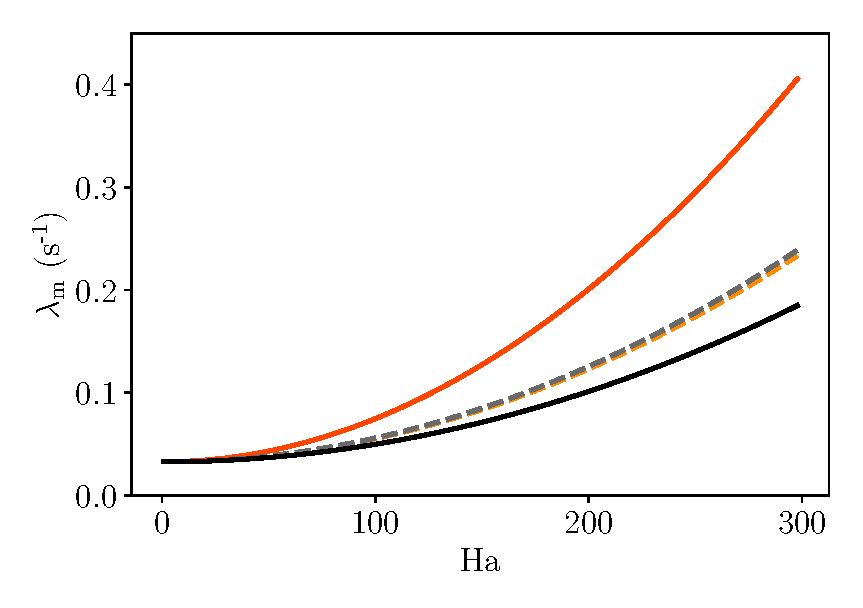
\includegraphics[width=0.48\linewidth]{figures/mag_damp_bc_20.eps} };
			\node (pic2) [right = 0cm of pic1]
			{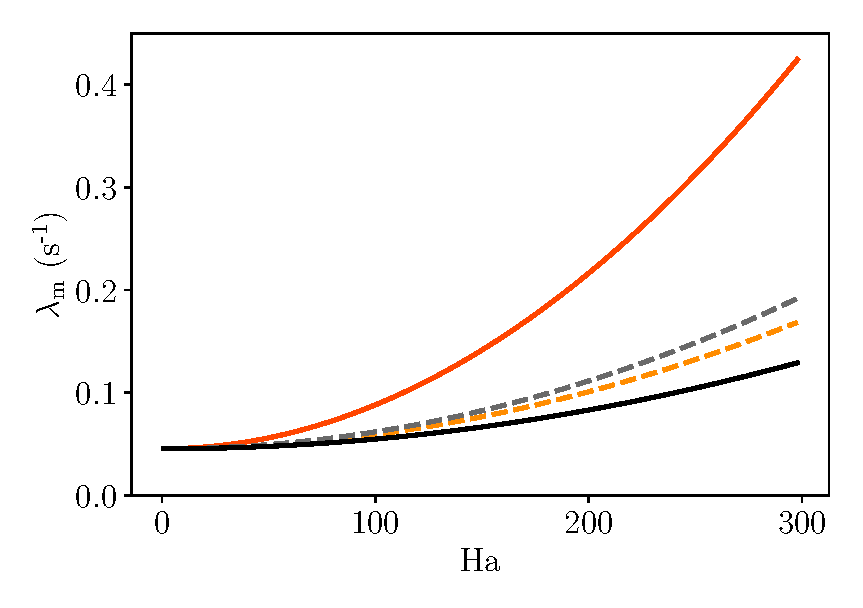
\includegraphics[width=0.48\linewidth]{figures/mag_damp_bc_11.eps} };
			\node (pic3) [below = 0.3cm of pic1]
			{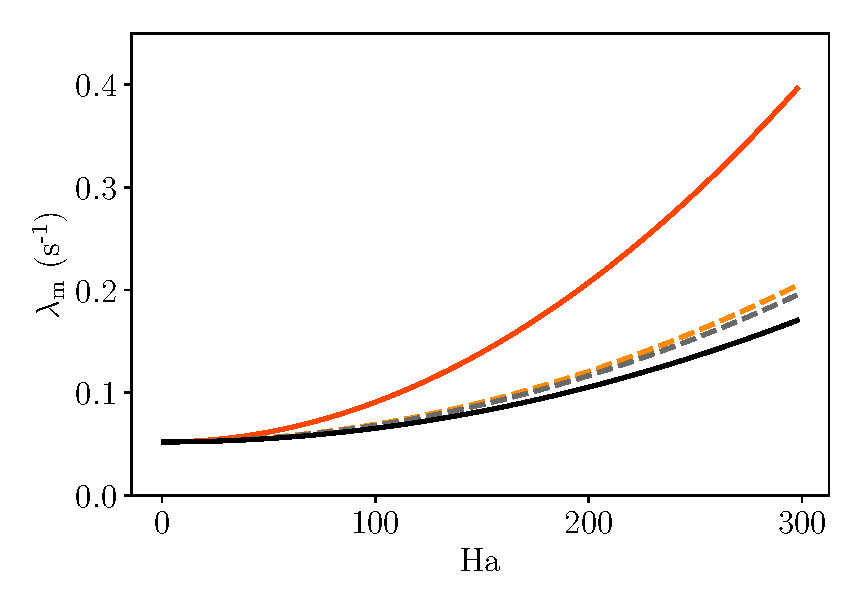
\includegraphics[width=0.48\linewidth]{figures/mag_damp_bc_21.eps} };
			\node (pic4) [right = 0cm of pic3]
			{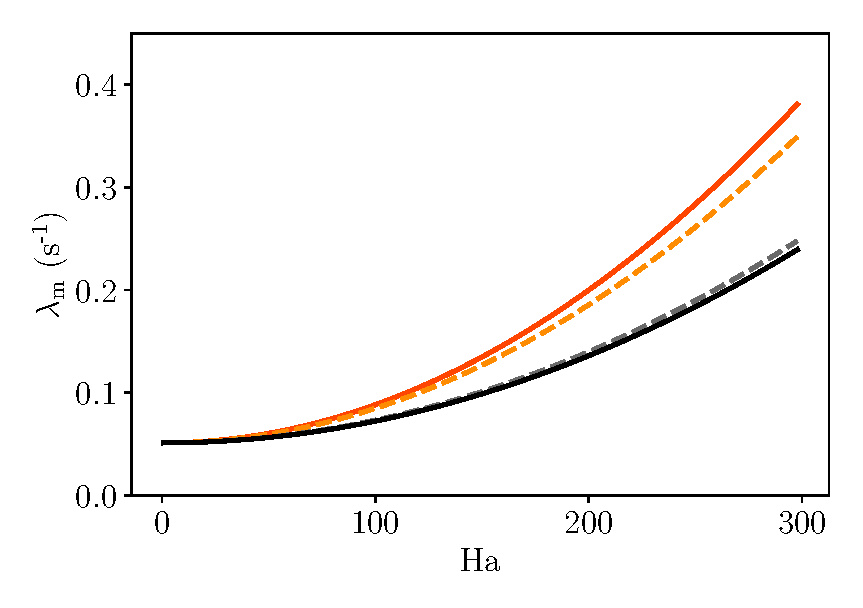
\includegraphics[width=0.48\linewidth]{figures/mag_damp_bc_12.eps} };
			\node (a) [above left = -2cm of pic1, yshift=1.2cm] {(a)};
			\node (b) [above left = -2cm of pic2, yshift=1.2cm] {(b)};
			\node (c) [above left = -2cm of pic3, yshift=1.2cm] {(c)};
			\node (d) [above left = -2cm of pic4, yshift=1.2cm] {(d)};
			
			\node [right = 0cm of a] {mode $(2,0)$:};
			\node [right = 0cm of b] {mode $(1,1)$:};
			\node [right = 0cm of c] {mode $(2,1)$:};
			\node [right = 0cm of d] {mode $(1,2)$:};
		\end{scope}
		
		\begin{scope}[yshift=-9.6cm,]
			\coordinate (x1) at (0,0);
			\coordinate (x2) at (0.75,0);
			
			\draw [ultra thick, orangered] (x1) -- (x2) node [right, black] {B.C 1};
			\draw [dash pattern=on 5pt off 3pt, 
			ultra thick, darkorange, transform canvas={xshift=2.3cm}] (x1) -- (x2) node [right, black] {B.C 2};
			\draw [dash pattern=on 5pt off 3pt,
			ultra thick, dimgrey, transform canvas={xshift=4.8cm}] (x1) -- (x2) node [right, black] {B.C 3};
			\draw [ultra thick, k, transform canvas={xshift=7.3cm}] (x1) -- (x2) node [right, black] {B.C 4};
		\end{scope}
		
	\end{tikzpicture}
	\caption{The analytical magnetic damping rates at different $\rm Ha$ of a single-layer system with different electrical boundary condition mentioned in Table\,\ref{tab:table_sim}. The wave modes considered are a) $(2,0)$, b) $(1,1)$, c) $(2,1)$ and d) $(1,2)$. The cell dimensions and material properties of the fluids are given in Table\,\ref{tab:table_bojarevics_prop}.}
	\label{fig:mag_damp_bc}
\end{figure}
%%%%%%%%%%%%

The total magnetic damping rate due to both the Ohmic dissipation given in Eq.\,\eqref{eq:mag_damping_rate_short} and the boundary layer given in Eq.\,\eqref{eq:tot_damping_Ha+Sh} is equal to the sum of the damping rates due to ohmic dissipation and boundary effects:
\begin{equation}
	\lambda_{\ii m} = \lambda_{\ii o} + \lambda_{\rm b}.
	\label{eq:mag_damping_rate}
\end{equation}

To show how the electrical boundary conditions affects magnetic induction, we calculate the magnetic damping rate of a system similar to \citet{Bojarevics2006a} (refer to Table\,\ref{tab:table_bojarevics_prop} for material properties). We calculate the magnetic damping rate at different $\rm Ha$ of a uni- and bidirectional free surface wave in four separate domains with the aforementioned boundary conditions. Figs.\,\subref{fig:mag_damp_bc}{a}, \subref{fig:mag_damp_bc}{b}, \subref{fig:mag_damp_bc}{c} and \subref{fig:mag_damp_bc}{d} represent the damping rates of the wave modes $(2,0)$, $(1,1)$, $(2,1)$ and $(1,2)$ within a range $0\leq \rm Ha \leq 300$, accordingly. 
The initial vertical offset at $B_z=\SI{0}{\milli\tesla}$ is due to the viscous dissipation at the walls. The damping behavior of B.C 1 and 4 is as expected, with current recirculation in the walls aiding and recirculation within the walls reducing Ohmic dissipation. The conducting sidewalls in B.C 1 provides a low-resistance bypass for the electric currents, whereas in B.C 4, the induced currents are forced to go through the highly resistive shear layer near the walls. This is known to reduce the total current flow in the fluid. The mixed boundary cases of B.C 2 and B.C 3 show contrasting behavior depending on the wave mode. In B.C 2, the configuration of the wave with respect to the orientation of the conducting plates plays a big role in determining the damping rate. A larger mode index in the $y$-direction ($n\!>\!m$) results in increased eddy current flow into the conducting plates oriented normal to the $x$-axis, thereby increasing the damping rate. Conversely, the damping rate reduces when $m\!>\!n$. This can be seen in Figs.\subref{fig:mag_damp_bc}{c} and \subref{fig:mag_damp_bc}{d} in relation to B.C 2. In B.C 3, the presence of a conducting bottom wall increases the overall Ohmic and boundary dissipation compared to an insulating bottom wall. This is in conformity with the experimental observations of \citet{Dominguez2017}, who considered a similar boundary configuration for swirling flows. Moreover, we also note that the damping curves of B.C 2, B.C 3 and B.C 4 converge to that of B.C 1 for very large wave modes, for all $B_z$ values.  
\\
\indent From the results presented above, it is clear that much of the damping is dictated by Ohmic dissipation, with boundary layer dissipation being comparatively small. Furthermore, it is evident that the nature of standing waves, uni- or bidirectional, the electrical boundary condition and its orientation with respect to the wave in some cases, along with the dimensions of the domain, affects the way in which the electric currents complete their paths within the medium and thus, determines the extent of magnetic damping.  



\subsection{Verification with \citet{Sreenivasan2005}}
\label{sec:sreeni_compare}

We now independently validate our formula for magnetic dissipation with the experimental results and analytical model presented by \citet{Sreenivasan2005}, which pertains to the decay of free surface waves in shallow rectangular geometries. Table\,\ref{tab:table_sreeni_prop} provides details on the physical parameters and material properties used for the study. \citet{Sreenivasan2005} have dedicated an entire study to the magnetic attenuation of standing gravity waves in rectangular containers and measured the decay rates of surface waves in liquid mercury that were exposed to vertical magnetic fields of up to  $\SI{1300}{\milli\tesla}$. Moreover, the authors provide a theoretical solution for magnetic damping times that takes into account bulk Ohmic dissipation, viscous side wall dissipation and Hartmann layer dissipation (at the bottom). The damping times are given by $\lambda_{\rm m}^{-1} = (\lambda_{\rm o}+\lambda_{\rm b})^{-1}$, also expressed as the inverse of the magnetic damping rate. Their model was the first to properly address the delicate problem of electrically insulating walls (B.C 4), but was only formulated for the first unidirectional wave mode $(m=1,n=0)$ using the shallow-water approximation. Fig.\,\ref{fig:sreeni_comp} shows the total damping time as a function of the Hartmann number, which in this context is given by $\ii{Ha} = B_zL_y\sqrt{\sigma/(\rho\nu)}$. At the shallow water limit ($kh\ll1$), the damping rate due to the viscous-Hartmann layer given in Eq.\,\eqref{eq:Ha_damp_topbot} transforms to 
\begin{equation}
	\lambda_{\rm Ha}
	= 
	\frac{\nu}{2\sqrt{2}\:h}
	\dfrac{1}{\sqrt{\tau\nu}}
	\sqrt{1 + \sqrt{1 + \tau^2\omega^2} }.
	\label{eq:sreeni_ha_damp}
\end{equation}
Even though \citet{Sreenivasan2005} does not consider dissipation at the Shercliff layers, we take this opportunity to formulate the damping rate
\begin{equation}
	\lambda_{\rm Sh} = \frac{\nu}{\sqrt{2} \;L_y}
	\frac{1}{\sqrt{h\sqrt{\tau\nu}}}
	\sqrt{ 1 + \sqrt{1 + \frac{\tau}{\nu}h^2\omega^2 }}
	\approx 
	\frac{\sqrt{\omega\nu}}{\sqrt{2} \;L_y}
	,
	\label{eq:sreeni_sh_damp}
\end{equation}
which is approximately equal to the hydrodynamic viscous damping rate at the sidewalls. Eqs.\,(\ref{eq:qind}, \ref{eq:qcorr_bc4}, \ref{eq:sreeni_ha_damp} and \ref{eq:sreeni_sh_damp}) together coincide with the Ohmic dissipation, Hartmann and viscous layer contributions from Eq.\,37 given in \cite{Sreenivasan2005}. This is shown in Figs.\,\subref{fig:sreeni_comp}{a} and \subref{fig:sreeni_comp}{b}, where we find good agreement between both theories and experiments at two different layer depths: \SI{22}{} and \SI{35}{\milli\meter} respectively. 

\begin{table}%[H] add [H] placement to break table across pages
	\caption{Cell parameters and material properties from \citet{Sreenivasan2005}.}
	\label{tab:table_sreeni_prop}
	\begin{ruledtabular}
		\begin{tabular}{llll}
			
			Length of cell ($L_x$): & \SI{0.15}{\meter}  &
			Wave mode $(m,n)$: & $(1,0)$
			\\
			Breadth of cell ($L_y$): 	& \SI{0.04}{\meter}  &
			Boundary condition: & Perfectly insulating walls. 
			\\
			& & & (similar to B.C 4)
			\\[5pt]
			Properties of Mercury ($\Omega$) &  &  & \\
			Density ($\rho$):
			& \SI{13546}{\kilogram\per\meter\tothe{3}} & Electrical conductivity ($\sigma$):
			& \SI{1e6}{\siemens\per\meter}
			\\
			Kinematic viscosity ($\nu$):
			& \SI{1.15e-7}{\meter\tothe{2}\per\second} & Layer depths ($h$): &
			\SI{0.022}{\meter}, \SI{0.035}{\meter}
		\end{tabular}
	\end{ruledtabular}
\end{table}
\begin{figure}
	\begin{tikzpicture}
		\node (pic1) at (-5,0) 
		{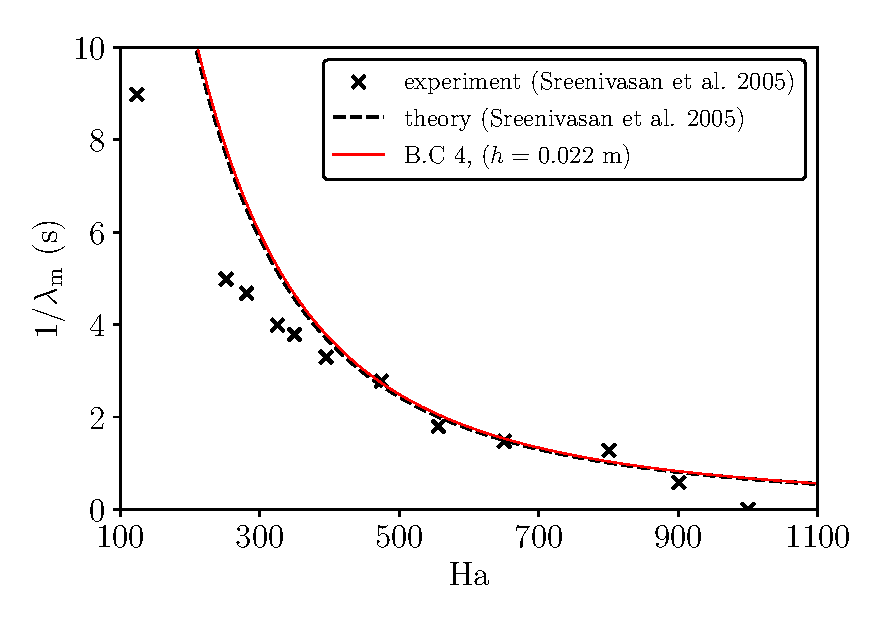
\includegraphics[width=0.5\linewidth]{figures/sreeni_damp_22mm.eps} };
		\node (pic2) at (3.8,0)
		{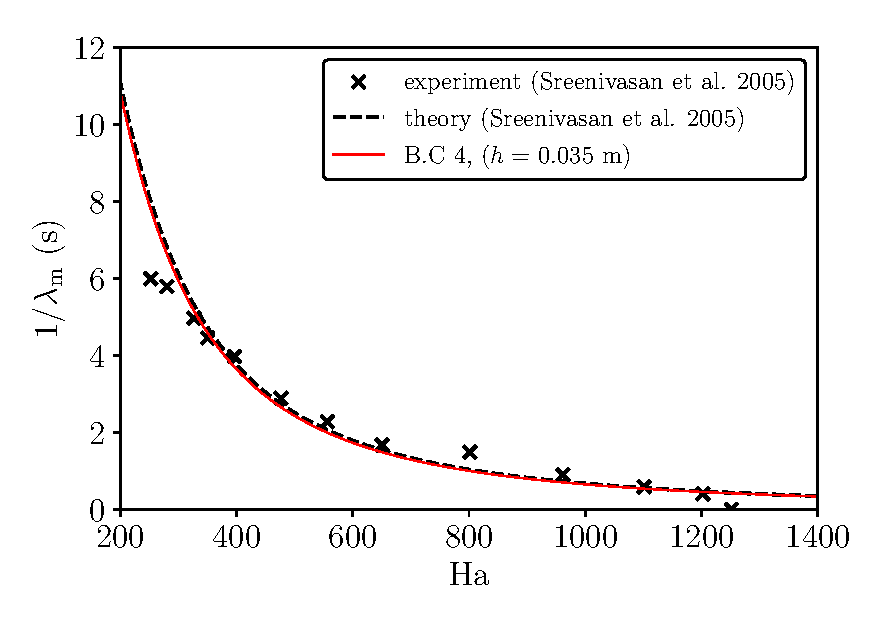
\includegraphics[width=0.5\linewidth]{figures/sreeni_damp_35mm.eps} };
		\node [above of=pic1, xshift=-4.1cm, yshift=2cm] {(a)};
		\node [above of=pic2, xshift=-4.1cm, yshift=2cm] {(b)};
	\end{tikzpicture}
	\caption{Comparison of the magnetic damping time which is the inverse of the magnetic damping rate  $\lambda_{\rm m} = \lambda_{\ii o^*} + \lambda_{\ii v^*}$, with experimental measurements and theoretical predictions of \cite{Sreenivasan2005} as a function of the Hartmann number $\rm Ha$ at two different layer depths: a) $h=\SI{0.022}{\meter}$ and b) $h=\SI{0.035}{\meter}$ of the liquid metal. The wave mode of the free surface wave was $(1,0)$.}
	\label{fig:sreeni_comp}
\end{figure}


\section{The magnetic damping experiment}
\label{sec:mag_damp_exp}

We now compare our analytical magnetic damping model from Sec\,\ref{sec:ohmic_dissipation} using a similar experimental setup from \citet{Hegde2025}. As in \cite{Sreenivasan2005}, we excited the free surface of a single-layer system and then proceeded to measure the rate of decay of the amplitude. We operated at a significantly lower range of $100 < \rm Ha < 500$, in contrast to \citet{Sreenivasan2005}. A standing wave of mode $(1,0)$ was magnetohydrodynamically excited using horizontal, externally fed currents. Exciting higher wave modes posed a challenge with the current setup, as these modes rely on the formation of distinct excess current loops within the liquid metal. This can only be achieved by vertically injecting the input current, which is not possible with the current configuration. Of the four different cases covered in the study, only B.C 1 and B.C 4 were realised in the experiment. The experimental setup and results are given in Sec.\,\ref{sec:exp_setup} and \ref{sec:exp_exp} respectively. 



\begin{table}
	\caption{Material properties of the working fluid and system parameters used in the magnetic damping experiment.}
	\label{tab:table_exp_prop}
	\begin{ruledtabular}
		\begin{tabular}{llll}
			
			Length of tank ($L_x$): & \SI{0.255}{\meter}  &
			Wave mode $(m,n)$: & $(1,0)$
			\\
			Breadth of tank ($L_y$): 	& \SI{0.255}{\meter}  &
			Boundary condition: & \Rn{1}) Copper plates on sidewalls (B.C 1). 
			\\
			Height of tank ($H$): & \SI{0.1}{\meter}  & & 
			\Rn{2}) Stainless steel plates on sidewalls (B.C 4)
			\\[5pt]
			Properties of GaInSn ($\Omega$) &  &  & \\
			Density ($\rho$):
			& \SI{6345}{\kilogram\per\meter\tothe{3}} & Electrical conductivity ($\sigma$):
			& \SI{3.2e6}{\siemens\per\meter}
			\\
			Kinematic viscosity ($\nu$):
			& \SI{3.4e-7}{\meter\tothe{2}\per\second} & Layer depth ($h$):
			& $\SI{0.03}{\meter}$
			\\[5pt]
			Properties of copper &  &  & \\
			Size: & $0.23\times 0.1 \times 0.002\,\SI{}{\meter\tothe{3}}$ &
			Electrical conductivity: & \SI{58e6}{\siemens\per\meter}
			\\[5pt]
			Properties of stainless steel &  &  & \\
			Size: & $0.23\times 0.1 \times 0.002\,\SI{}{\meter\tothe{3}}$ &
			Electrical conductivity: & \SI{1.1e6}{\siemens\per\meter}
		\end{tabular}
	\end{ruledtabular}
\end{table}

%%%%%%%%%%%%%%%%%
\begin{figure}
	\begin{tikzpicture}
		\node (pic1) at (-5,0) 
		{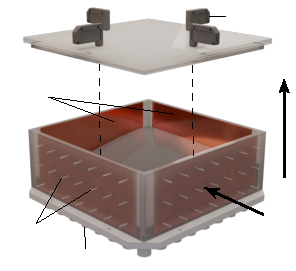
\includegraphics[width=0.5\linewidth]{figures/exp_render.pdf} };
		\node (pic2) at (3.5,0)
		{\includegraphics[width=0.45\linewidth]{figures/curr_profile.eps} };
		\node [above of=pic1, xshift=-3.9cm, yshift=2.2cm] {(a)};
		\node [above of=pic2, xshift=-3.7cm, yshift=2.2cm] {(b)};
		
		%labels
		\node (txt1) at (-7.95,1.2) [left] {metal plates};
		\node [below of=txt1, yshift=0.65cm] {(copper/steel)};
		
		\node at (-7.5,-2.8) [left, yshift=-0.5mm] {connectors};
		
		\node at (-6.8,-3.4) [below] {sensor mount};
		\node (dist) at (-2.7,3.6) [right] {distance};
		\node [below of=dist, yshift=0.6cm] {sensor};
		
		\node at (-0.9,1.7) [above] {$B_z$};
		\node (curr) at (-1.5,-2.4) [right, xshift=-0.5mm, yshift=-0.6mm] {$-I_y$};
		
		
		
		\node at (-5,-0.5) {GaInSn};
		
		%		% Grid
		%		\draw[lightgray,step=0.5] (pic1.south west) grid (pic1.north east);
		%		
		%		% Axes' labels
		%		\foreach \x in {-9.5,-9,...,-0.5} { \node [below] at (\x,0) {\x}; }
		%		\foreach \y in {-4,-3.5,...,4} { \node [left] at (0,\y) {\y};}
		%		axis
		
		%axis
		\draw [-Stealth, very thick] (-5,3) -- (-5.7,2.8) node [xshift=-1mm]{$x$};
		\draw [-Stealth, very thick] (-5,3) -- (-4.3,2.8) node [xshift=1mm]{$y$};
		\draw [-Stealth, very thick] (-5,3) -- (-5, 3.7) node [yshift=1mm]{$z$};
		
	\end{tikzpicture}
	\caption{(a) A 3D rendering of the experimental setup where a standing wave is generated either in the $x$- or $y$-direction by passing current $I_y$ or $I_x$ respectively, through the four metal plates on the sidewalls. (b) depicts the current waveform $I_y$ or $I_x$ for a given time period ($2\pi/\omega$) required to excite a standing wave with resonant frequency $\omega$. The dimensions of the tank are $L_x=\SI{0.255}{\meter}$, $L_y=\SI{0.255}{\meter}$ and total height $H=\SI{0.1}{\meter}$. }
	\label{fig:exp_model}
\end{figure}
%%%%%%%%%%%%%


\subsection{The setup}
\label{sec:exp_setup}

The specifications of the experimental setup are provided in Table\,\ref{tab:table_exp_prop}. The wave tank was made out of polymethyl methacrylate (PMMA) with inner dimensions of $0.255 \times 0.255 \times 0.1\,\SI{}{\meter\tothe{3}}$. The walls were $0.008\,\SI{}{\meter}$ thick. Each of the inner faces of the four sidewalls had a cut to facilitate the insertion of metal plates $0.23 \times 0.1 \times 0.002\,\SI{}{\meter\tothe{3}}$ in size. As shown in Fig.\,\subref{fig:exp_model}{a}, the metal plates did not extend fully along the length of the PMMA wall, but had a small gap of $0.0125\,\SI{}{\meter}$ from either end, to prevent short circuits. The metals in question were copper and stainless steel depending on the required electrical boundary condition, as explained below in Sec.\,\ref{sec:exp_exp}. Each metal plate was welded with 21 uniformly placed shunt resistors, protruding outwards. The combination of thin plates and the shunts ensured a homogeneous current density needed to excite a linear standing wave. The entire tank was vertically placed at the center of a Helmholtz coil generating a quasi-homogeneous vertical magnetic field $B_z$ up to $\SI{50}{\milli\tesla}$ across the wave tank. The tank was filled with GaInSn, a eutectic alloy of Ga, In and Sn which is liquid at room temperature, up to a height of $\SI{0.03}{\meter}$. The rest was filled with Argon gas, to hinder the oxidation of GaInSn due to contact with ambient air. Distance sensors were placed on top of the tank as well as at the bottom, at four locations along the $x$- and $y$-axis, to simultaneously measure the instantaneous wave amplitude. 


\subsection{The experiment}
\label{sec:exp_exp}

\begin{figure}
	\begin{tikzpicture}
		\node (pic1) at (-5,0) 
		{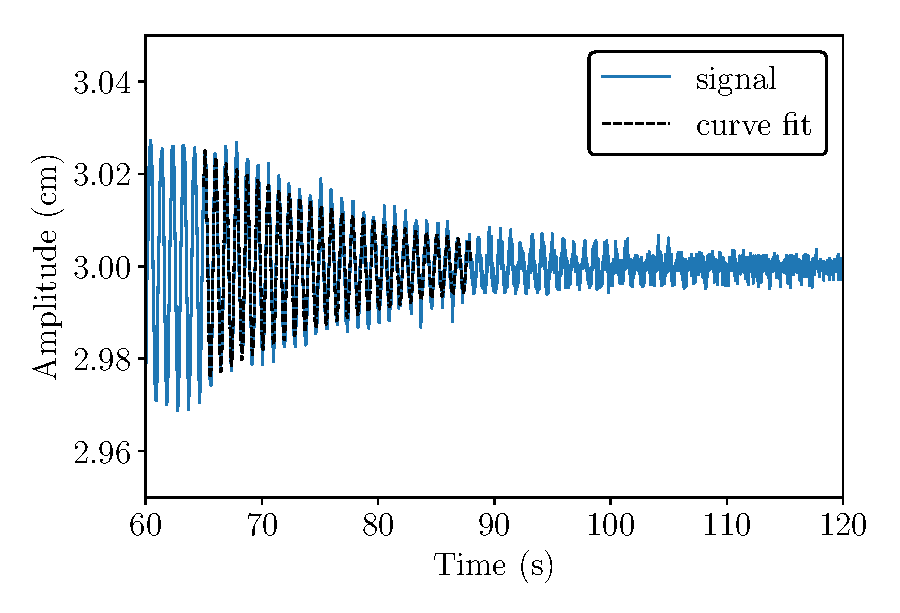
\includegraphics[width=0.5\linewidth]{figures/vlog.eps} };
		\node (pic2) at (3.8,0)
		{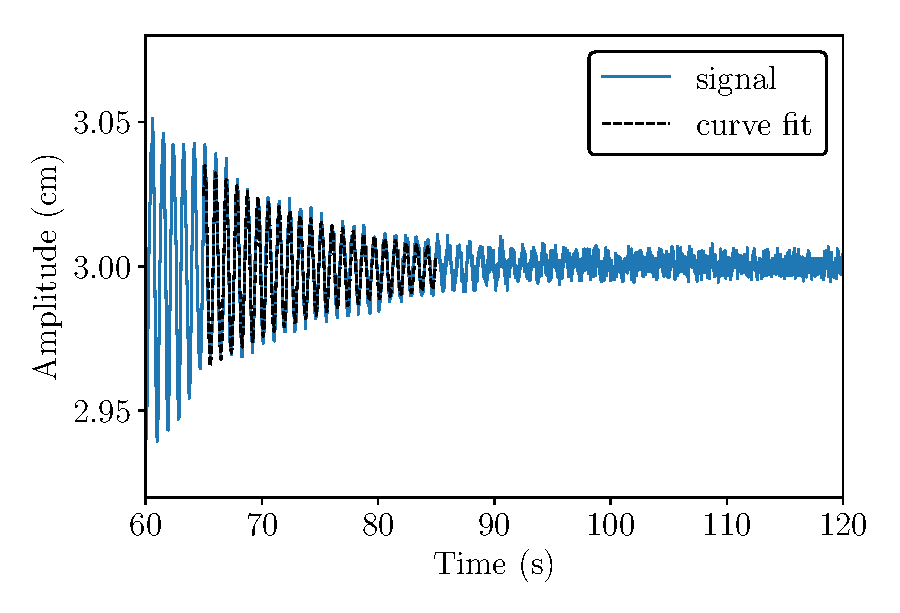
\includegraphics[width=0.5\linewidth]{figures/tlog.eps} };
		\node [above of=pic1, xshift=-4.1cm, yshift=1.8cm] {(a)};
		\node [above of=pic2, xshift=-4.1cm, yshift=1.8cm] {(b)};
		
		\node at (4.6,-1) {$\lambda_{\rm m} = \SI{0.0807}{\per\second}$};
		\node at (-4.2,-1) {$\lambda_{\rm b}
			 \approx \SI{0.0624}{\per\second}$};
		
	\end{tikzpicture}
	\caption{The amplitude decay profile of wave mode $(1,0)$ in a square wave tank with stainless steel sidewall inserts, a) without the presence of a vertical magnetic field $B_z$ and horizontal current $I_y$ and b) in the presence of a magnetic field $B_z=\SI{20}{\milli\tesla}$ ($\rm Ha = 196$) without horizontal current. At low $\rm Ha$, we can ignore the effects of the Hartmann layer and consider the damping contribution at the boundary to be purely hydrodynamic. The difference between the total damping and the boundary layer contributions yields the  damping rate due to Ohmic dissipation $\lambda_{\ii o}=\SI{0.018}{\per\second}$.}
	\label{fig:post_process}
\end{figure}

\begin{figure}
	\begin{tikzpicture}
		\node (pic1) at (-5,0) 
		{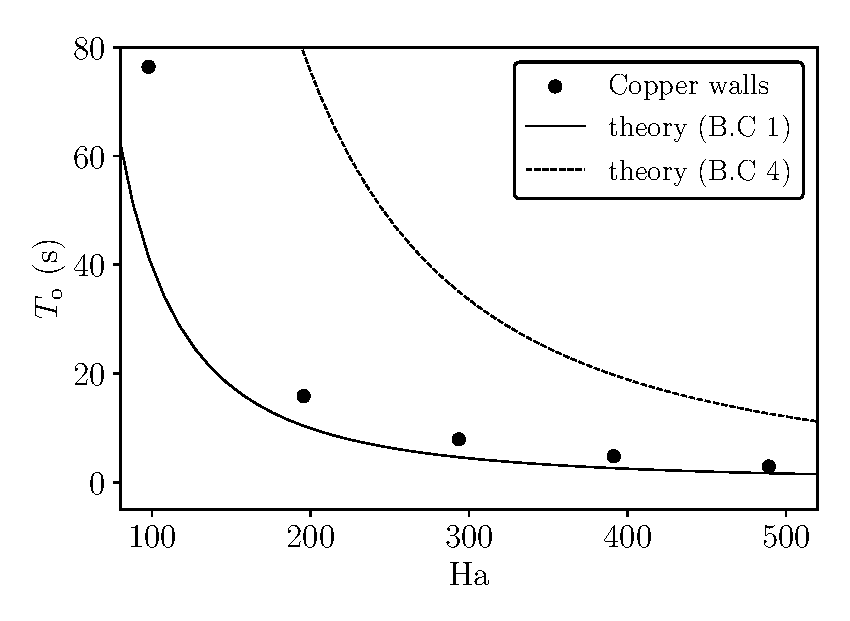
\includegraphics[width=0.5\linewidth]{figures/mdamp_h3_cm_copper_time.eps} };
		\node (pic2) at (3.8,0)
		{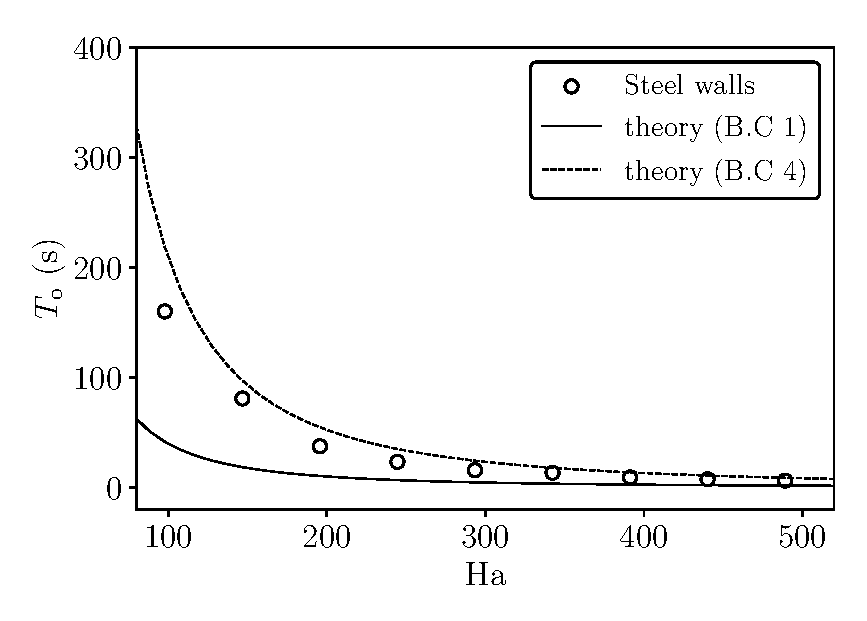
\includegraphics[width=0.5\linewidth]{figures/mdamp_h3_cm_steel_time.eps} };
		\node [above of=pic1, xshift=-4.1cm, yshift=2cm] {(a)};
		\node [above of=pic2, xshift=-4.1cm, yshift=2cm] {(b)};
	\end{tikzpicture}
	\caption{The comparison of theoretical and experimental damping times $T_{\rm o} = \lambda_{\ii o}^{-1}$ due to Ohmic dissipation in a wave tank with a) copper sidewalls (B.C 1), and b) stainless steel sidewalls (B.C 4) at different $\rm Ha$. For the theoretical calculation, copper walls are treated as perfect conductors and stainless steel walls as perfect insulators.}
	\label{fig:exp_results}
\end{figure}

The free surface of the liquid metal is excited when a horizontal current is supplied to the GaInSn across any two parallel metal plates in the $x$- or $y$-axis, in the presence of a constant vertical magnetic field $B_z$. To generate a quasi-1D standing wave of mode $(1,0)$ with a resonant frequency $\omega$, a proportional current signal as shown in Fig.\,\subref{fig:exp_model}{b}, must be given in the $y$-direction. The time period of the signal $T=2\pi/\omega$ and the size of the wave is proportional to the amplitude of the signal. Because we magnetohydrodynamically excite the wave, we are limited to using electrically conducting materials in the sidewalls. To simulate conducting and insulating sidewalls, we make use of copper (Cu-ETP) and nickel-plated stainless steel. As given in Table\,\ref{tab:table_exp_prop}, GaInSn is significantly less conductive than copper, by a factor of about twenty, and has a conductivity that is three times that of stainless steel. Therefore, copper walls act as a relative conductor (B.C 1) and stainless steel walls as a relative insulator (B.C 4). 
\\
\indent We conduct the experimental measurements between $\rm Ha=100$--$500$ ($B_z=10$--\SI{50}{\milli\tesla}). From Fig.\,\ref{fig:stokes_vel}, we know that at lower values of $\rm Ha$, the effect of the magnetic field on the velocity gradient at the wall boundary layer is negligible. This means that the dissipation due to boundary effects can be considered as a purely hydrodynamic phenomenon and that any field-induced change is dominated by Ohmic dissipation. This allows us to isolate the contribution of Ohmic dissipation to the total damping measured, which is one of the main results of the present study. The following steps were used to achieve this: \Rn{1}) we first excited a wave using an oscillating current signal $I_y$ and magnetic field $B_z$. After a certain amount of time ($t=\SI{60}{\second}$) after the wave was properly developed, both the current and magnetic fields were switched off and the amplitude of the wave was recorded with respect to time. The slope of this decaying signal gives us the viscous damping rate $\lambda_{\rm v}$, as the energy of the wave is dissipated solely due to viscous effects at the boundary. \Rn{2}) Subsequently, a wave was excited again, but only the input current $I_y$ was cut off after a given time to initiate wave decay. The slope of the decaying amplitude signal gives the magnetic damping rate $\lambda_{\rm m}$, which takes into account both the Ohmic dissipation and the boundary layer effects [Eq.\,\eqref{eq:mag_damping_rate}]. We have already established that the boundary layer effects with and without the magnetic field are the same, $\lambda_{\ii b}\approx\lambda_{\ii v}$. The difference $\lambda_{\rm m} - \lambda_{\rm v}$ is the Ohmic damping rate $\lambda_{\ii o}$ and the inverse $T_{\rm o}=\lambda_{\ii o}^{-1}$, the Ohmic damping time for a particular $\rm Ha$. Fig.\,\subref{fig:post_process}{a} and \subref{fig:post_process}{b} provides an example of the extraction of $\lambda_{\rm o}$ from $\lambda_{\ii b}$ and $\lambda_{\rm m}$ respectively at $\rm Ha=196$ ($B_z=\SI{20}{\milli\tesla}$) in a tank with stainless steel sidewalls. The Ohmic damping rate/time is independent of the initial amplitude of the wave.
\\
\indent  Fig.\,\ref{fig:exp_results} contains the experimental results and compares $T_{\rm o}$ measurements in a tank with copper and stainless steel sidewalls, at different values of $\rm Ha$ with the theoretical cases B.C 1 and B.C 4. We present the results in terms of damping times in order to remain consistent with the previous literature \cite{Sreenivasan2005}. We saw good agreement in both cases, where the measurements done for the waves in copper and stainless steel sidewalls closely follow the theoretical damping times of B.C 1 and B.C 4 cases respectively. As seen in Fig.\,\subref{fig:exp_results}{a} and Fig.\,\subref{fig:exp_results}{b}, the slight overshoot in the measurements with copper walls and the undershoot with stainless steel walls was expected. The metal inserts have a certain amount of thickness ($d=\SI{2}{\milli\meter}$) and are neither perfect conductors nor insulators.
\\
\indent The damping times at higher depths, i.e. $h=0.04, 0.05$ and $\SI{0.06}{\meter}$ were also measured, but revealed no considerable change in the values. It was not possible to achieve greater depths due to limited wall height of the tank, and the risk of GaInSn splashing outward and damaging the top-mounted distance sensors. 


\section{Concluding remarks}
\label{sec:conclusion}
In this work, we have developed a theoretical description of the magnetic damping of standing free-surface waves in rectangular containers. The formulation extends previous approaches for shallow, one-dimensional waves to arbitrary one- and two-dimensional standing-wave modes at finite depth, and to a range of homogeneous and mixed electrical boundary conditions. We derived analytical solutions for the induced electric potential and current distributions, and used them to determine the Ohmic dissipation and the corresponding magnetic damping rates. In addition, we formulated the modification of the oscillating boundary layers by the magnetic field, including both Hartmann and Shercliff layers.

A central result is the strong influence of the electrical boundary conditions on the induced current paths and, consequently, on the magnetic damping rate. For conducting walls, the induced currents can close through the walls, whereas insulating boundaries force them to recirculate within the liquid, thereby reducing the total current and Ohmic dissipation. For mixed electrical boundary conditions, the damping additionally depends on the orientation of the conducting boundaries relative to the wave mode. This becomes particularly relevant for two-dimensional standing-wave modes, for which increasingly complex current patterns develop. For an arbitrary mode $(m,n)$, the induced horizontal current distribution consists of $(m+1)(n+1)$ eddies. The total magnetic damping further contains a contribution from the magnetically modified boundary layers. Within the range of parameters considered here, this contribution is mainly affected by the Hartmann layer, while the influence of the Shercliff layer on the sidewall dissipation remains negligible.

The analytical formulation agrees well with the shallow-water theory and experiments of \citet{Sreenivasan2005}. We further validated the predicted Ohmic damping experimentally for non-shallow waves using conducting and insulating sidewalls. By performing the measurements at comparatively low Hartmann numbers, the magnetic modification of the boundary-layer damping remained small, allowing the Ohmic contribution to be isolated directly from the measured decay rates.

Accurate damping rates are particularly important for the prediction of magnetohydrodynamic wave instabilities such as the metal pad roll instability. Their onset is governed by the competition between electromagnetic excitation and the dissipation of the interacting wave modes. A reliable stability prediction therefore requires the damping rates of these modes to be known with comparable accuracy. In our recent MPR theory for small-scale models \cite{Hegde2026}, viscous damping rates were derived together with analytical expressions for the resulting growth rates and instability thresholds. The present formulation provides the corresponding magnetic damping contribution and thereby completes the damping description required for the linear prediction of MPR instability.

Future work should particularly address the experimental validation of two-dimensional standing-wave modes and mixed electrical boundary conditions. Such measurements would provide a direct test of the more complex current distributions predicted by the present model and further establish its applicability to coupled-wave instability problems.

% If you have acknowledgments, this puts in the proper section head.
\begin{acknowledgments}
	This study was supported by Deutsche Forschungsgemeinschaft (DFG, German Research Foundation) by Award No. 512131026. The authors would like to thank Michael Knobel for the chemical treatment, Klaus Timmel for the mechanical design, Bernd Nowak for the construction of the wave tank and William Nash for proofreading the manuscript.
\end{acknowledgments}




% Specify following sections are appendices. Use \appendix* if there
% only one appendix.

\appendix*
\section{Modeling the Hartmann layer at the interface of a two-layer stratified fluid system}
\label{app}

In a two-layer stratified system with varying density $\rho_1 < \rho_2$ and large conductivity difference $\sigma_1\ll\sigma_2$, the phenomenon of induction largely remains the same as outlined in Secs.\,\ref{sec:elec_potential} and \ref{sec:eddy_current}. However, the modeling of boundary layer dissipation is distinct due to the incorporation of an additional boundary, the interface. A free surface is allowed to slide freely and therefore, has zero shear stresses. This is not the case in an interface between two liquid mediums. Here, tangential velocity and tangential stress are continuous, but the velocity gradients generally differ
because the dynamic viscosities differ. This leads to the formation of a interfacial Hartmann layer where the tangential induced currents coupled with the vertical magnetic field $B_z\h e_z$ produce Lorentz forces which balance the mechanical tangential stresses. In liquid-liquid systems where $\sigma_1\ll\sigma_2$, the Hartmann layer forms at the interface of the better electrical conductor. To model the dissipation of energy due to the interfacial Hartmann layer, we write the following balance equations:
\begin{subequations}
	\begin{gather}
		\h u_{1,\perp}|_{\mathcal S} = \h u_{2,\perp}|_{\mathcal S},
		\label{eq:interface_tang_vel}
		\\
		p_2|_{\mathcal S} - p_1|_{\mathcal S} =
		(\rho_2-\rho_1)g\eta + 2(\rho_2\nu_2\partial_z u_{2,z} - \rho_1\nu_1\partial_z u_{1,z}),
		\label{eq:young_laplace_eq}
		\\
		\rho_1\nu_1(\partial_z u_{1,x} + \partial_x u_{1,z})|_{\mathcal S}
		=
		\rho_2\nu_2(\partial_z u_{2,x} + \partial_x u_{2,z})|_{\mathcal S},
		\label{eq:tangent_stressX}
		\\
		\rho_1\nu_1(\partial_z u_{1,y} + \partial_y u_{1,z})|_{\mathcal S}
		=
		\rho_2\nu_2(\partial_z u_{2,y} + \partial_y u_{2,z})|_{\mathcal S}.
		\label{eq:tangent_stressY}
	\end{gather}
\end{subequations}
Here, Eq.\,\eqref{eq:interface_tang_vel} refers to the continuity of the tangential velocity at the interface $\mathcal{S}$, where the suffix ($\perp$) denotes the tangential component of each fluid layer. Secondly, Eq.\,\eqref{eq:young_laplace_eq} is the modified Young-Laplace equation which captures the hydrostatic balance considering normal stresses at the interface. Lastly, Eqs.\,(\ref{eq:tangent_stressX}--\ref{eq:tangent_stressY}) show the continuity of the tangential stresses at the interface. 
\\
\indent To deduce the tangential velocities in the Hartmann layer on either sides of the interface, we make use of the boundary conditions\,(\ref{eq:tangent_stressX} and \ref{eq:tangent_stressY}) to satisfy
\begin{equation}
	{\h u}_{1,\perp} +  {\bar{\h u}}_{1,\perp}|_\mathcal{S} 
	\approx
	{\h u}_{2,\perp} +  {\bar{\h u}}_{2,\perp}|_\mathcal{S} 
	\qquad
	\begin{cases}
		\rho_1\nu_1\partial_z{\bar{u}}_{1,x}|_\mathcal{S} 
		\approx
		\rho_2\nu_2\partial_z{\bar{u}}_{2,x}|_\mathcal{S} \\[5pt]
		\rho_1\nu_1\partial_z{\bar{u}}_{1,y}|_\mathcal{S} 
		\approx
		\rho_2\nu_2\partial_z{\bar{u}}_{2,y}|_\mathcal{S}
	\end{cases}\hspace{-3mm},
	\label{eq:interface_jump_condition}
\end{equation}
and subsequently obtain
\begin{align}
	{\bar{\h u}}_{1,\perp}|_{\mathcal S}
	&=
	\frac{\omega\Lambda}{k\sqrt{\rho_1\nu_1\sigma_1}
		\sqrt{1 + \sqrt{1 + \tau_1^2\omega^2} }
	}
	\begin{Bmatrix}
		\dfrac{m\pi}{L_x}
		\;\sin{\left[\dfrac{m\pi}{L_x}\left( x + \dfrac{L_x}{2} \right)\right]}
		\cos{\left[\frac{n\pi}{L_y}\left( y + \dfrac{L_y}{2} \right)\right]}
		\h e_x 
		\\[20pt]
		\dfrac{n\pi}{L_y}
		\;\cos{\left[\dfrac{m\pi}{L_x}\left( x + \dfrac{L_x}{2} \right)\right]}
		\sin{\left[\dfrac{n\pi}{L_y}\left( y + \dfrac{L_y}{2} \right)\right]}
		\h e_y
	\end{Bmatrix} \ii{e}^{-
		\dfrac{1}{\delta_{\rm tot}}
		z} ,
	\label{eq:Ha_int_up_velocity}
\end{align}
\begin{align}
	{\bar{\h u}}_{2,\perp}|_{\mathcal S}
	&=
	\frac{-\omega\Lambda}{k\sqrt{\rho_2\nu_2\sigma_2}
		\sqrt{1 + \sqrt{1 + \tau_2^2\omega^2} }
	}
	\begin{Bmatrix}
		\dfrac{m\pi}{L_x}
		\;\sin{\left[\dfrac{m\pi}{L_x}\left( x + \dfrac{L_x}{2} \right)\right]}
		\cos{\left[\frac{n\pi}{L_y}\left( y + \dfrac{L_y}{2} \right)\right]}
		\h e_x 
		\\[20pt]
		\dfrac{n\pi}{L_y}
		\;\cos{\left[\dfrac{m\pi}{L_x}\left( x + \dfrac{L_x}{2} \right)\right]}
		\sin{\left[\dfrac{n\pi}{L_y}\left( y + \dfrac{L_y}{2} \right)\right]}
		\h e_y
	\end{Bmatrix} \ii{e}^{
		\dfrac{1}{\delta_{\rm tot}}
		z} ,
	\label{eq:Ha_int_dwn_velocity}
\end{align}
where,
\begin{equation}
	\delta_{\rm tot} = \frac{\sqrt{2\tau_i\nu_i}}{\sqrt{1+\sqrt{1+\tau_i^2\omega^2}}}, 
	\qquad (\ii{from Eq.\,\eqref{eq:hartmann_layer_thickness}}),
\end{equation}
and $\Lambda$ given by
\begin{equation}
	\Lambda = A_{mn}\:\frac{(\text{coth}[kh_1] + \text{coth}[kh_2]) }
	{
		\dfrac{1}{\sqrt{\rho_1\nu_1\sigma_1}
			\sqrt{1 + \sqrt{1 + \tau_1^2\omega^2} }  }
		+
		\dfrac{1}{\sqrt{\rho_2\nu_2\sigma_2}
			\sqrt{1 + \sqrt{1 + \tau_2^2\omega^2} }  }
	}.
\end{equation}
\indent The tangential velocities help us in determining the tangential stresses which can be related to the strain rate. We use the same approach of \citet{Hegde2026} for a two-layer stratified system undergoing linear sloshing. Therefore, the new mechanical energy balance reads:
\begin{equation}
	\dv{}{t}\left( \sum_{i=1,2} \frac{1}{2} 
	\int_{V_i} \rho_i \norm{\h u_i}^2 \mathrm dV  \right)
	+
	\dv{}{t}\left( \int_{\mathcal{S}} 
	\frac{1}{2} (\rho_2-\rho_1)g\eta^2  \: \mathrm d\mathcal{S}  
	\right)
	= -\sum_{i=1,2} 2\rho_i\nu_i
	\int_{V_i} \bm\varepsilon_i \bm{\mathbin{:}} \bm\varepsilon_i  \: \mathrm dV ,
	\label{eq:balance_boundary_new}
\end{equation}
which is same as Eq.\,\eqref{eq:balance_boundary} but with the addition of the potential energy term  arising due to the interface. In a standing wave, the kinetic and potential energy have a phase difference of $\pi/2$. Solving the right hand side of Eq.\,\eqref{eq:balance_boundary_new} as shown in Sec.\,\RN{3} of the supplementary material \cite{SMmagdamp_hegde}, we get the damping rate at the interface:
\begin{equation}
	\lambda_{\rm int}=
	\frac{k}{2\sqrt{2}}
	\left(
	\frac{ \dfrac{1}{\xi_1\sigma_1\sqrt{\tau_1\nu_1}}
		+
		\dfrac{1}{\xi_2\sigma_2\sqrt{\tau_2\nu_2}} 
	}{ 
		\dfrac{\rho_1}{\text{tanh}[kh_1]} + \dfrac{\rho_2}{\text{tanh}[kh_2]} }
	\right)
	\left(
	\frac{
		\dfrac{1}{\text{tanh}[kh_1]} + \dfrac{1}{\text{tanh}[kh_2]} 
	}
	{
		\dfrac{1}{\sqrt{\rho_1\nu_1\sigma_1}\;\xi_1} + 
		\dfrac{1}{\sqrt{\rho_2\nu_2\sigma_2}\;\xi_2}
	}
	\right)^2,
	\label{eq:Ha_damp_int}
\end{equation}
where,
\begin{equation}
	\xi_i = \sqrt{1 + \sqrt{1 + \tau_i^2\omega^2} }, \quad \ii{and} \quad
	\tau_i = \frac{\rho_i}{\sigma_iB_z^2},  \quad \{i=1,2\}.
\end{equation}
Eq.\,\eqref{eq:Ha_damp_int} is the damping rate due to viscous and magnetohydrodynamic boundary layers at the interface of two-liquids with large conductivity difference. The upper layer of the interface is purely viscous whereas the lower layer constitutes the viscous and Hartmann layer.











% Create the reference section using BibTeX:

\bibliography{mag_damp}

\end{document}
%
% ****** End of file apstemplate.tex ******

